% Main Meaning Model theory manuscript.
\documentclass[11pt,a4paper]{article}

\usepackage[utf8]{inputenc}
\usepackage[longtitle]{emergentwisdom-preprint}
\usepackage{mathtools}
\usepackage{booktabs,tabularx,array,float}
\usepackage{enumitem}
\usepackage{xcolor}
\usepackage{graphicx}
\usepackage{tikz}
\usetikzlibrary{arrows.meta,positioning}
\usepackage{microtype}
\usepackage{hyperref}

\newcolumntype{Y}{>{\raggedright\arraybackslash}X}
% Canonical compact interface shared with the Life Simulation snapshot.
% Keep this file theory-only: no implementation or experiment claims.
\newcommand{\MMCoreSummary}{%
Six forms carry the world model: Concept, Thing, Event, Binding, Cut, and
Realization. Bindings give Things roles in Events, while typed links connect
records without turning every connection into the same relation. A Cut answers
one question by dividing one stated unit among exclusive alternatives and a
remainder; those shares total one. A Realization links a Concept to an
addressable fragment without a weight, and any graded fit is expressed by a
separate Cut on an assessment Event. The six forms keep identity, occurrence,
participation, decomposition, and grounding apart without claiming to exhaust
metaphysics. A construction profile may add lifecycle, admissibility, and
recomposition rules while retaining the same forms. Understanding Nodes and
Document Nodes share their address space with world records but keep distinct
authority and validation, and perspective follows declared authority ancestry rather than a
duplicated attribution field.%
}

\newcommand{\MMCoreSchema}{%
\begin{center}
\footnotesize\ttfamily
\begin{tabular}{@{}l@{}}
Concept \{ id, names, typed relations, constraints,\\
\qquad grounding records, provenance \}\\
Thing \{ id, kind, identity boundary, continuity criterion,\\
\qquad typed links, provenance \}\\
Event \{ id, kind, interval, typed world data, optional description,\\
\qquad direction, typed links, provenance \}\\
Binding \{ id, event, role, thing, interval, provenance \}\\
Cut \{ id, parent Event, question, profile, divided unit,\\
\qquad keyed weighted answers, keyed remainder, optional conditioning address,\\
\qquad constraints, provenance \}\\
Realization \{ id, purpose, context parent, target, concept,\\
\qquad grounding version, optional alignment, evidence, provenance \}
\end{tabular}
\end{center}
\noindent\footnotesize Answer and remainder addresses pair the Cut revision
with a local key; they are not additional record forms.\normalsize%
}

\newcommand{\MMProfileSummary}{%
In the selected profile, each Thing has one lifecycle Event spanning its
modeled existence. Active joint Events and their Bindings determine
encapsulation, so no second containment truth is stored. Every Cut declares the
unit it partitions, gives weights to exclusive answers and a remainder, and
totals one; sequential weights come from covered duration. Understanding and
Document Nodes can point into the same graph as the six world forms without
acquiring world authority. An Event description is optional text on the Event,
not a Document Node.%
}

\newcommand{\MMProfileSchema}{%
\MMCoreSchema
\begin{center}
\footnotesize\ttfamily
Profile Cut conventions \{ allocation, sequential, direction;\\
\qquad sequential shares derived from duration \}
\end{center}%
}


\hypersetup{
  hidelinks,
  pdftitle={The Meaning Model: Constructing Worlds and Stories at Progressive Resolution},
  pdfauthor={Henrik Westerberg},
  pdfsubject={A compact grammar and method for jointly constructing worlds, concepts, understanding, and stories at progressive resolution},
  pdfkeywords={meaning model, concept grounding, event decomposition, realization, finite resolution, recursive refinement}
}

\renewcommand{\shorttitle}{The Meaning Model}
\setlist[itemize]{leftmargin=1.4em}
\setlist[enumerate]{leftmargin=1.6em}

\title{The Meaning Model:\\Constructing Worlds and Stories at Progressive Resolution}
\author{Henrik Westerberg\\Emergent Wisdom\\
  \texttt{henrik.westerberg@emergentwisdom.org}}
\ewreviseddates{September 5, 2026}{October 3, 2026}

\begin{document}
\maketitle

\begin{abstract}
The Meaning Model proposes a shared medium for constructing a world, its meanings,
interpretations in Understanding Graphs, and stories, reports, or programs, with
the long-term aim of modeling reality computationally through interrelated
processes, from physical and social histories to attributed inner life, at a
declared finite resolution. Without prior measurement, a language model's
implicit understanding, already attached to reality through human writing, can
become explicit, comparatively quantified, and recursively constructible before
evidence tests it. Unmeasured histories get comparative commitments rather than
freestanding scores: a Cut, one of six record forms, divides a declared unit under
a question into exclusive answers and an explicit remainder. Processes carry them
as trajectories that generation must consult and preserve or revise, the proposed
mechanism for consistent thinking and acting. Records and discovered concepts can
anchor new inference and abstraction; developing and revising the categories
themselves is part of the construction method.

Its two linked architectural contributions, progressive resolution and a shared
construction medium, form one coordinated authoring method, not a new record type
or the storage of prose beside a graph: a world is built coarse and opened
recursively where a declared purpose needs detail, and each opening preserves
declared commitments or explicitly revises them, with their dependent accounts and
passages. The medium is a candidate training language for choosing, deepening, and
repairing representations. Life Simulation develops the construction-to-learning
loop; this paper specifies the representation and preservation contracts. The
completed \emph{Book of Conditions} partly demonstrates construction feasibility
but does not validate the full method; learning gains, computational
savings, and alignment remain untested.
\end{abstract}

\keywords{Meaning Model, Recursive World Grammar, Concept Grounding,
Event-Processes, Progressive Detail, Finite Resolution}

\section{Introduction}

Reality does not arrive already divided into every ``thing'' to which people
give a word. We identify a person's life, an expedition within that life, a
marriage, an avalanche, a species, a recession, and a story. Each term makes
some portion or pattern of experience addressable while leaving other
variation in the background. The same evening of reading can belong to a
person's biography, a book's history, human culture, biological evolution, and
the physical history of Earth.

A revolution or the growth of a city can be represented with the same grammar
as a single evening: participants, phases, and processes that change one another
at different timescales. A century of city growth can open into migrations,
building projects, and individual decisions; each can be decomposed again where
the inquiry needs it. Trust and legitimacy need no standard physical unit.
Relations can remain unweighted; where numerical comparison is useful, shares
answer a declared question about a divided whole. Money, population counts, and
duration keep their own units, whether they are measured, inferred, or authored
during construction.

A boundary alone does not preserve reference. The same person may participate
in a life, an expedition, a rescue, and a later conversation; those events need
a stable way to state that they concern the same continuing individual.
Conversely, a person may be opened into organs, cells, or devices for one
question without discarding person-level identity. The difficulty is therefore
not producing one description, but preserving identity and meaning when a
description is opened, revised, compared with another world, or rendered into
language. Ordinary prose can silently change what a term refers to. A flat
graph can store relations without stating how coarse and fine descriptions
agree. An unqualified numerical rating can preserve neither who attributed it
nor the comparison or measurement protocol that gives it meaning.

The Meaning Model proposes one grammar for those responsibilities. Reusable
Concepts describe continuing Things and Events. A Cut divides one stated unit
among answers to a question: for example, how a character's attention is shared
among current concerns, with a remainder for unresolved allocation. Bindings state
which Thing fills which role in an Event, and a Realization records an attributed
claim that a fragment of the world instantiates a Concept. A Concept
may remain lightly specified or have a process-based model written in the same
grammar. Finer articulation reuses the same identities and respects existing
commitments. The \emph{modeler} is the person or AI system constructing,
interpreting, or revising this account; \emph{constructor} names its role when
proposing changes, and the \emph{generator} is the component producing
candidates. These name roles, not additional record forms.

Behind the design is a question: what must be rendered for a simulated world to be
believable to whoever experiences it? A reader, a viewer, or a player probes a
world only locally, through one route, one scene, or one visit. The world
therefore need not be detailed everywhere. It needs a coarse but consequential
account of its macro-processes, the long developments, institutions, economies,
and environments within which lives and events happen, and detail opened
wherever attention or the purpose reaches, each opening consistent with what the
coarse account commits. Believability then comes from causal coherence across
scales rather than from uniform detail: whatever the experiencer probes follows
from the larger structure. Level-of-detail simulation asks a related question
about computation and perception~\cite{brom2007,sunshine2010}; here the question
extends to meanings, inner lives, and text. It is progressive resolution seen
from the experiencer's side, with the declared resolution set by what the
experiencer can reach and what the purpose needs.

The central idea is that this construction is possible at all. Many world models
admit a quantity only after measurement, so an unmeasured history, such as one
character's trust in another over a year, stays qualitative. A language model,
however, is already attached to reality through its implicit conceptual
understanding, learned from human writing about the world. Because that
understanding was learned from language, questions can draw much of it out in
words, and the accompanying tool is built to ask them
(Section~\ref{sec:modeling-workflows}). The model can therefore make its own
understanding explicit and recursively constructible, including particular
histories nobody measured and concepts nobody has named, before evidence tests
the account. The written account need not be faithful to be useful: it is
attributed, inspectable, and testable, so its errors can be found and corrected
instead of staying latent.

Explicit structure does more than record that understanding: it is the proposed
mechanism for consistent thinking and acting. Processes carry trajectories over
time; states nobody measured receive comparative shares under a declared
question and unit, with an explicit remainder, instead of an invented absolute
scale, as when, in the Book's authored reading, Babbage's outlook at the trial of
May 1851 divides into assurance .76, threat .18, and an unresolved .06; and the
grammar keeps with every claim whose account it is and what it concerns. These
trajectories are explicit commitments that generation must consult and then
preserve or revise: when the model writes a scene, makes a character decide, or
changes a program, it is to read the recorded state of each relevant process at
that moment instead of improvising from its context. The same numbers make a
proposed refinement checkable by arithmetic, as double-entry bookkeeping catches
an inconsistency without establishing that the books are true, and because the
records persist, another agent or a later session can inspect, correct, and build
on them. A language model that carries out the construction the tool instructs is
meant to build coherent worlds and books this way. \emph{The Book of
Conditions} was begun under the author's direction while the tool itself was being
built, and its later revisions were made through the tool. Whether works built
this way are more coherent than unstructured writing is what the prospective
evaluation tests. The method is
designed for programs too: a code unit is a DocumentNode that could be linked to
the processes and concepts it implements, so that a change to the model would
name the code it puts in question, though no program has yet been built this way.
The numerical-dependence test in Section~\ref{sec:prospective-evaluation} is
designed to measure whether the numbers actually steer what the model writes.

In principle, nothing in the method needs a computer. A novelist could have written every
character's life from childhood, tracked each voice and belief as a process with
comparative numbers, and linked every sentence to the Events it depicts. The
balance of costs has likely kept authors from doing so. One continuous mind can hold
much of a novel's world implicitly, while writing that understanding down,
keeping it current, and linking it to the text would take more work than most
books can bear. Tacit knowledge also resists telling: ``we can know more than we
can tell''~\cite[p.~4]{polanyi1966tacit}, which made knowledge acquisition the
bottleneck of knowledge engineering~\cite{feigenbaum1977art}. Where one mind was not enough, as in series bibles,
writers' rooms, and franchise continuity, the explicit record has usually been
kept only as far as the work required. A language model changes the balance.
Extensive articulation can become far easier for it, while it lacks a continuous
mind to hold a long work together, so persistent records supply continuity
across sessions and agents that its context cannot. What is new is what this makes
possible: progressive resolution and a shared construction medium connect
discovered concepts, quantitative commitments, recursive refinement, and
coordinated revision in one inspectable account.

Construction is also a method of discovery. The intended agentic use is to give
an intelligent system a small, recursively
reusable toolbox for building an explicit world model. A common objection holds
that language models lack world models, and that intelligent systems must
instead learn predictive world models directly~\cite{lecun2022path}. The
Meaning Model takes a different route: rather than requiring a network to learn
a world model internally, the language model constructs an explicit one from
what it has learned, which can then be inspected, tested, and revised. A language model can
draw on learned world knowledge to infer and make explicit the processes,
motives, relationships, and quantities behind events, including what people
know implicitly but have not recorded or measured. Each explicit record becomes
an anchor for further inference: the constructor can connect records, infer
higher-level concepts from their relationships, and open those concepts into
finer processes. Beginning from an institution that is losing legitimacy, for
example, it may infer inconsistent decisions, unequal access, and failed
expectations that nobody has measured. Those records can support a concept of
procedural betrayal, which may then guide the study of another institution or
explain a character's changing loyalties. The resulting structure anchors
another round of abstraction and refinement; neither the domain, conceptual
vocabulary, nor depth is fixed in advance. The system can also discover where
its current account is inadequate, propose finer structure or a better
decomposition, and test the change against observations or generated
consequences. Useful changes should survive without losing the identities,
meanings, and history already accepted; conflicts require explicit revision.
The toolbox supports the growth of the conceptual space, not just
relationships among concepts supplied in advance. Discovering and revising
person categories through joint human and AI construction is part of this work,
not merely an option to replace a finished inventory.

Progressive resolution and a shared construction medium are the proposal's two
linked architectural contributions. They are also the machinery the central idea
needs:
progressive resolution lets an anchor be opened without losing what is already
committed, and the shared medium lets a discovered concept be revised together
with its instances, reasons, and prose. Together they form one construction method,
in which world commitments, concept interpretations, authoring reasons, and prose
are refined and revised together, and each opening preserves declared
commitments or revises them explicitly. Four representational changes carry it:

\begin{itemize}
  \item \textbf{Construct detail under commitments.} A useful world can precede
    its finer history. An opening preserves declared coarse answers or makes
    the necessary revision explicit; it does not merely reveal precomputed detail.
  \item \textbf{Revise the account across surfaces.} World state, abstract concept
    models, Event descriptions, document text, and externalized understanding
    participate in one authoring operation. Exact dependencies identify which
    interpretations, reasons, and passages a changed commitment puts in question.
  \item \textbf{Construct meanings as well as instances.} A concept can be
    articulated through the same roles and processes as a situation that realizes
    it. Definition, application, and revision become inspectable operations,
    without requiring deep grounding for every concept.
  \item \textbf{Give semantic numbers their comparison context.} A coherent
    comparative question avoids requiring an absolute scale for each abstract
    concern. Its numbers describe a concept's contextual role rather than an
    intrinsic quantity, retaining the question, alternatives, remainder, and
    perspective.
    Measurements keep external units; concurrent processes do not become shares
    merely because they describe one person or world.
\end{itemize}

The running example is \emph{The Book of Conditions}, a completed alternate
history in which Babbage's bounded calculating apparatus is built and put to
work by a calculation office. Its commercial organizer, Edward Halden, accepts
orders beyond the office's independent checking capacity, while Lovelace seeks
a successor to sustain that checking. In 1854 an unchecked, erroneous table is
delivered: the story concerns the human and institutional conditions of a
computational claim, not just whether the machine works.

Refinement should preserve \emph{semantic continuity}. Starting from the coarse
claim that Babbage builds an Engine, a construction may later expose the
machine's parts, its workforce, or competing accounts of the work without
changing which Babbage, Engine, or building process earlier records addressed.
Unopened regions can remain coarse; openings must fit the accepted boundary
or revise it visibly. Suppose a coarse account calls an apparatus trial
successful under a criterion requiring every case to pass on the first
uninterrupted run, and its explanation and passage depend on that assessment.
Opening the trial into phases introduces a stopped run followed by a successful
restart. Those phases cannot be accepted as mere detail: they contradict the
protected criterion, so the constructor must reject the opening or propose an
explicit revision. A narrower claim, complete agreement after restart, would
require a new grounding version, a revised assessment, a reason for the
change, and rechecking the dependent passage, while the earlier account remains
addressable. This hypothetical cycle shows the contract; it is not a recovered
transaction from the Book. Section~\ref{sec:construction-protocol} states the record-level
acceptance rules.

The same contract connects a character's modeled concerns to decisions and
scenes. Comparative numerical accounts of wants and appraisals should guide a
decision before its scene is written. Opening the decision can expose a
conflict with those concerns or with what the character knows; the modeler can
then revise the action, or revise the concept used to interpret it, while
retaining the reasons and rechecking the scene. The immediate value is a
working model that helps a modeler investigate what happens and why, and decide
what to construct next. In storytelling, it guides decisions before prose rather
than merely cataloguing a finished story. A whole life or institution can be sketched first, then
opened where its decisions and consequences matter; incompatible detail prompts
revision of the larger account.

\subsection{Uses and long-term aims}

The long-term theoretical aim is a representation that could model reality
computationally through interrelated processes, including people's inner lives,
at a declared finite resolution. The grammar is a representational substrate
rather than an annotation shell around a finished simulator, and a model is
complete only relative to a declared question and resolution. Domain-specific
processes, measurements, and laws may be attached without becoming new universal
record forms. The larger aim is representational compression: to describe
everything meaningfully distinguishable at declared finite resolution with as
few domain-neutral operations as possible, so that a new domain adds content
rather than a universal primitive. This ambition concerns progressive
articulation of any part of reality or possibility that a purpose makes
relevant, not computation of all reality at maximum detail. Minimality concerns
the responsibilities a validator must preserve, not the world's ultimate
furniture.

The representation is intended as a general-purpose modeling medium. Narrative worlds,
simulation and knowledge systems, corpus annotation, and perspective-separated
accounts of people are applications of the same grammar; storytelling supplies
the first worked application here, not a boundary on the method. These uses fall
into two families that share the construction loop: generating something new,
such as stories, game worlds, and ideas, and describing something that exists,
such as a market, an institution, or a person's own life. Each use needs
stable reference, attributed claims, and compatible resolutions; the grammar
alone does not guarantee their practical benefit. For interactive worlds, the
same method could leave much of the world coarse but consequential. A
regional harvest failure can constrain a town's supply before its warehouses and
households are constructed. A player's visit opens one warehouse, then a
worker's experience of the shortage, under the protected supply commitments and
domain rules. This is construction of previously absent detail, not selective
display of a finished simulation. Distant events can still require coarse
updates, later visitors must encounter a history compatible with recorded
observations and intervening changes, and shared facts cannot silently change
between players. Whether this saves computation at comparable fidelity
remains untested by the Book.

These uses admit two complementary deployment modes. An intelligent system can read and update the
records as an explicit semantic workspace. By returning to earlier numerical
accounts and the questions or explanations linked to them, it could develop
continuity of understanding across interactions: what changed, what might
explain it, and whether the change belongs to the world or to its own estimate.
The same distinctions and construction histories can also become prediction and
reconstruction targets: a candidate training language for learning to choose
useful distinctions and revise an account, not only assign values within a
fixed vocabulary. Operating such models could become partly internal to the
learner, while explicit records remain available for persistence, correction,
and inspection; the learner need not reproduce their syntax internally.

The scope includes attributed inner life. Beliefs, feelings, wants, and private
interpretations may be represented without turning a character's report, an
observer's estimate, and accepted public state into one claim: accepted world
Events descend from History, while an attributed interior Event additionally
descends through the relevant person's lifecycle and inner-process root. This
ancestry preserves the boundary without making private experience directly
observable or selecting one universal psychology. The
long-term ambition is a model with increasingly accurate intuitions for a
person's inner life: what someone wants, fears, believes, and feels, and how
those processes shape decisions over time. Considering how to imitate an adult
mind, Turing pointed to ``the process which has brought it to the state that it
is in'': the mind's initial state, the education it received, and its other
experience~\cite{turing1950computing}. The representation models a person the
same way, from where their life processes begin, through what they were taught,
to what else they lived through, and construction asks for that history where it
explains who the person became. Better measurement data and more capable models
should make those estimates closer to the person being modeled, with
improvement assessed against later evidence. Each person's account of the world
can be represented beside the accounts others hold of that person and a shared,
evidence-supported world model. The aim is to understand how people decide from
the worlds they perceive, including what they misunderstand or leave unsaid,
rather than treating a shared description as everyone's view.

\subsection{Scope of the claim}

The claim has two parts that must not be confused.

\begin{itemize}
  \item \textbf{Recursive refinement} is a property of the world grammar:
    every finer articulation uses the same records and the local contracts of
    its declared construction profile. A deeply grounded concept may reuse that
    grammar in a process-based concept model, but need not do so.
  \item \textbf{Finite-resolution sufficiency} is a constructive hypothesis:
    for a declared purpose and tolerance, the distinctions required by the
    task can be represented through those records without claiming that the
    representation is unique, complete at every resolution, or mechanically true.
\end{itemize}

The central idea stated at the start of this Introduction rests on both and adds
an empirical expectation: that explicit construction improves on what a language
model does implicitly. Section~\ref{sec:prospective-evaluation} states how it is
tested.

The paper also plays, deliberately, with a stronger idea: that a person's inner
state, their wants, feelings, beliefs, attention, and outlook, and more broadly
the processes of a world, can be described at a declared resolution as a set of
numbers that change over time, and that the set can be opened into ever finer
detail. Nobody has recorded hundreds of such variables across a whole life,
because nobody needed to; a language model can now construct them. The paper
adopts this as a working hypothesis to explore, not as a result. Its numbers are
comparative shares under declared questions, not intrinsic intensities, and they
sit beside qualitative processes and relations that carry no numbers. Whether
such a description predicts what a person does, or what a reader recognizes as
true to them, is what the evaluation and Life Simulation are designed to test.

The construction discipline belongs to this paper: frozen-parent whole
candidates, direction rolls, atomic commit or rejection, explicit revision,
rendering routes, and read-back. Life Simulation develops methods for
generating, advancing, inferring, and learning process histories, including when
to open detail and how to test its predictive value; compact temporal laws are
optional~\cite{westerbergLifeSimulation2026}. The two proposals operate
throughout an ongoing construction: Life Simulation can propose a change, while
the Meaning Model specifies how to represent, accept, or revise its commitments.
The proposal also combines explicit character-state modeling before prose with
recursive conceptual decomposition from Fractal Intelligence
\cite{westerbergFractal2026}. Fractal Intelligence decomposes capabilities and
problems: child Solvers inherit constraints, their
combined result is evaluated against the caller's acceptance criteria, and a
failure may challenge the parent's framing. The Meaning Model applies a related
responsibility to world accounts: finer records must reconstruct protected
coarse answers or revise the commitments explicitly. Both permit recursive
decomposition without a fixed depth limit, while each actual construction or
execution remains finite.

Section~\ref{sec:grammar} states the grammar and its progressive construction,
Section~\ref{sec:concepts} concepts and their grounding, and
Section~\ref{sec:interop} the linked surfaces, transactions, rendering, and
read-back. Section~\ref{sec:closure} turns recursive refinement into a
finite-resolution sufficiency test. Section~\ref{sec:book-construction} reports
the Book and the prospective evaluation, and
Section~\ref{sec:modeling-workflows} the current workflows.
Section~\ref{sec:implications} considers what changes if works are constructed
this way. Sections~\ref{sec:related} and~\ref{sec:limitations} relate the proposal to
prior work and state its limits, and Section~\ref{sec:companion} places it in
the wider research program.

\begin{center}
\fbox{\begin{minipage}{0.90\linewidth}
\textbf{The minimized core of the grammar.}
\MMCoreSummary
\end{minipage}}
\end{center}

\section{Grammar and Progressive Construction}
\label{sec:grammar}

In the Book's current model, the apparatus trial of May 1851 shows the six
forms together. Babbage, Lovelace, the apparatus, and the sealed test packet are
Things with continuing identities. The trial is an Event, opened into a first run
that stops and is begun again, a second complete run that agrees with the sealed
independent results, and a few idle cycles of shared pleasure; Bindings
place it at its site, and a spatial child Event binds the people and objects
present. An Event beneath Babbage's inner process carries a Cut dividing his
outlook toward his active wants into assurance (.76), threat (.18), and a
remainder (.06), an authored reading rather than a probability.
\emph{Valid computational claim} is a Concept, and a Realization records the
claim that the trial instantiates it. The trial's protocol required the stop and
voided the incomplete run, so no commitment had to be revised; the
Introduction's hypothetical cycle shows what the contract requires when one
must be. The rest of this section states what each form is responsible for and
how a world built from them is opened.

The core is minimized at the level of record forms, not vocabulary labels. It
uses six forms---Concept, Thing, Event, Binding, Cut, and Realization---and
introduces a new form only when no existing form plus typed fields can preserve
a distinction that a validator must enforce. This is relative minimality under
the declared contract, not a proof of globally minimal syntax or metaphysical
primitives.

The definitions and rules needed to use this account are stated in this paper;
the separately typeset \emph{Minimized Grammar} collects them as a compact
reference without adding requirements or changing their status.

Each form answers a question that the others cannot answer without erasing a
distinction or relocating its responsibility. A Concept says which reusable
meaning is intended. A Thing says which continuing instance is addressed. An
Event says what persists or occurs.
A Binding says which Thing fills which time-scoped role. A Cut says how one
declared unit divides under one question. A Realization says which Concept
grounds an addressable world fragment. The fragment is a subgraph of existing
records rather than a seventh world form.

The removal test concerns these responsibilities, not their serialization.
Removing Thing identity requires another way to join a person's appearances;
removing Binding requires another way to distinguish that person's roles;
removing Realization requires another way to distinguish a concept definition
from its application. The same test applies to occurrence and allocation.
Another schema may combine these forms while retaining equivalent typed
information. Thus six is a compact, inspectable interface, not a lower bound
on every possible encoding; complexity in field types and validators counts
against the claim just as additional record forms would.

\MMCoreSchema

A reference distinguishes a logical identity from an exact record revision.
In the selected immutable profile, an edit creates a successor revision, not a
new Thing or Concept identity. Provenance records the author or generator,
commit, construction time, and evidence references. Times name their clock:
Event chronology, construction history, or document order. Derived views retain
their source revisions and derivation lineage rather than acquiring independent
authority.

Relations are carried in four ways. A Binding assigns a Thing a typed,
time-scoped role in an Event. A Cut relates a parent to weighted child answers
and a remainder under one question and unit. Typed relation fields connect
Concepts, Events, records, or typed world-data fields under declared kinds. A
Realization grounds a world fragment in a Concept for a declared purpose. Each carrier retains the target,
authority, clock, inference, and validation contract of its relation kind.

A relation among several Things is consequently a joint Event with one Binding
per role, not a direct binary edge between the Things. Typed links such as
\texttt{contains}, \texttt{about}, \texttt{updates}, and \texttt{supersedes}
are sibling kinds, not synonyms. \texttt{contains} asserts scoped
Event--Event containment; \texttt{about} is reference without participation or
state change; \texttt{updates} names an affected process or typed world-data
field changed by an Event; and \texttt{supersedes} preserves a predecessor while changing a
typed lineage. A supersession must name its scope and clock, because replacing
a character's earlier belief in story time is not the same authority operation
as superseding an author note or a model commit in construction time.

A Realization is an attributed, unweighted grounding link. A \emph{define}
realization associates a Concept with a grounding model or family; a
\emph{describe} realization applies a recorded grounding version to a fragment.
For example, the first links helping to its definition, and the second links a
particular interaction to that definition. Each link retains a context parent
(an Event or surface node), provenance, available evidence, and any role
alignment. The relation is many-to-many across Concepts, fragments, perspectives,
and times.

A graded judgment uses a separate assessment Event linked \texttt{about} its
target beneath the process whose perspective it expresses. Its local Cut
divides the comparison unit among \emph{matches}, \emph{does not match}, and
remainder. Separate Concepts use separate fit Cuts; no independent Realization
degree is introduced. Every Cut is parented by an Event, even when the target
of assessment is a Concept or another record.

Cut answers are addressable components: a reference names the Cut revision and
a stable local answer key, even at zero weight; the remainder has its own
reserved key. An answer's
target and its component address are distinct, since the same Event may answer
several questions. Nested Cuts name the particular component whose conditional
unit they divide. Conditioning addresses must resolve and cannot form cycles.
This supplies exact targets for refinement, grounding, and notes without adding
another world record form.

The query contract is ancestry-complete within the caller's authorized view.
Only declared authority-parent edges confer context: \texttt{context-parent}
links and containment links explicitly assigned that role. They form an acyclic
graph. Traversal stops at the nearest declared context root on each path:
accepted-world, inner, understanding, document, or candidate. All such paths
must resolve to the same governing root; conflicting roots require separate
claims, not an arbitrary parent choice. Temporal ancestry is queried separately.

Access is checked before following an edge or returning its target. A denied
private reference reveals neither content nor private ancestry. Reference,
evidence, \texttt{renders}, and Realization target links do not grant access;
following \texttt{about} never changes perspective. A lookup returns the
permitted typed parent paths. A Cut or component lookup returns its parent
Event, question, unit, keyed siblings, conditioning address, remainder, and
recomposition rule together, or withholds that entire view. It never exposes
an isolated weight whose required context is inaccessible.

The parsimony rule admits a new primitive only when existing forms cannot preserve a distinction
in targets, composition, authority, inference, or validation. Helpful names may
be added; shared serialization never implies shared semantics.

\subsection{Optional construction profile}

The six forms play the role of a language; a construction profile selects how
to use it for a task. Treating the Book's categories as Meaning Model itself
would be like treating one Python script as Python. The intended practice is
to develop better vocabularies and decompositions, by humans and AI together,
judged by the characters and worlds they produce.

The six forms do not by themselves require one lifecycle convention, temporal
partition, or domain vocabulary. This paper uses a stronger profile to show how
they can construct a progressively resolvable world. Other profiles may choose
different children and depths or omit human modeling entirely. What remains
general is the Cut contract: when a decomposition uses a Cut, it names its
parent quantity and question, admits mutually exclusive answers under that question, retains a
remainder, and states how the answers reconstruct the parent.

The reading rule is simpler. A semantic number is a Cut weight: it means one
answer's share relative to its siblings under the parent Event's question and
unit, and the answers plus remainder sum to one. A non-summing process relation
is unweighted. Literal dates, durations, counts, currency amounts, positions,
and other quantities with independently interpretable units or declared
measurement protocols are typed Event data with units or protocol references
and provenance. They add neither a weighted Cut relation nor an unweighted process
parent relation. A Realization is likewise unweighted; optional
graded fit is represented by its own local Cut. If no divided unit and mutually
exclusive answers can be named, no semantic number is assigned.

Three Cut families---allocation, sequential, and direction---yield five named
profiles: facet, contribution, cause, sequential, and direction. Their
validator-visible distinctions are specified in Section~\ref{sec:normalized-cuts}.

The construction interface exposes six operation families. They are a small
authoring surface over the records, not six additional ontological primitives.

\emph{Register} stages an addressable Concept, Thing, or Event; in the lifecycle
profile a new Thing and its lifecycle enter the same candidate. \emph{Bind} assigns a
Thing a time-scoped role in an Event. \emph{Open or compose} is one structural
family with two retained modes: open refines a frozen authoritative parent,
whereas compose proposes a new parent over existing Events. \emph{Cut} adds
question-relative answers under one declared profile. \emph{Decide} rejects a
candidate, commits it as new, or commits an immutable revision that records
superseded targets and revalidates its dependency closure. \emph{Realize}
defines or describes Concept grounding while retaining purpose, version,
context parent, evidence, and uncertainty.

These operations make explicit structure a basis for further inference. The
modeler can open an existing account into finer processes, compose a higher-level
account from existing Events, or propose a concept model that makes a newly
inferred pattern addressable. The resulting structure can anchor another round
of construction.

Convenient construction names specialize those families without enlarging the
record grammar.

\begin{table}[htbp]
\centering
\small
\begin{tabularx}{\textwidth}{@{}p{0.19\textwidth}p{0.28\textwidth}Y@{}}
\toprule
\textbf{Construct} & \textbf{Core or interface basis} & \textbf{Why the name remains} \\
\midrule
Facet, contribution, cause & Allocation Cut & Their answer eligibility, interpretation, and validation differ \\
Presence, membership, part--whole & Event plus typed Bindings & Their roles and interval constraints support different queries and validators \\
Update & Event plus \texttt{updates} link & It asserts an effect on a process or typed world datum rather than generic reference \\
Supersession & Typed \texttt{supersedes} link & Its scope and clock determine which lineage changes authority \\
Roll & Direction Cut plus Decide & The original forecast, seed, fixed mass, drawn mass, and alternatives must survive selection \\
Roster, inherited presence, summaries & Read-only derivations & They follow from committed records and carry derivation lineage rather than new authority \\
Understanding, render, read back & Understanding and document workflow & They operate on linked text surfaces outside the six world-record forms \\
\bottomrule
\end{tabularx}
\caption{Named conveniences built on the minimized record grammar.}
\label{tab:construction-specializations}
\end{table}

Five cross-record rules govern this profile.

\begin{enumerate}
  \item Nonnegative, mutually exclusive Cut-child weights and the explicit
    remainder sum to one under the declared question and unit.
  \item Qualified decompositional refinement satisfies its profile-specific
    composition operator within tolerance, or the candidate is rejected or
    committed as an explicit revision.
  \item Containment and sequential children respect their applicable parent
    temporal or spatial extent; direction candidates instead respect the
    forecast horizon and are not treated as present parts.
  \item Every active Binding interval lies inside its Event and the lifecycle
    of each actively participating Thing; an \texttt{about} link does not
    imply participation.
  \item A Cut inherits the governing authority context of its parent
    Event; a different perspective requires another attributed Event beneath
    the corresponding typed root and another Cut.
\end{enumerate}

A concrete construction may add stronger gates, such as co-presence checks or
a rationale requirement for selected changes, provided it declares them; they
are not universal laws of every domain represented by the core.

\subsection{Progressive world construction}

The optional profile used here adds lifecycle anchoring and conservative
refinement to the core. It is one way to build a world, not a requirement of
every Meaning Model.

\subsubsection{Roots, identity, and relations}

The profile distinguishes two roots. The Universe is a Thing that addresses the
continuing identities in scope. History is its lifecycle Event and contains the
accepted Events within the declared horizon. Time is carried by Event intervals
and typed temporal data, not represented as another Thing. Merely assigning a
date to a candidate does not place it in accepted History.

Each Thing names an identity boundary, a continuity criterion, and exactly one
lifecycle Event in this profile. The Engine may therefore remain the same Thing
while its location, ownership, completion, parts, and social interpretation
change. An active participant Binding must lie inside the participant's
lifecycle. Later Events may still refer to a destroyed machine or a dead person
through \texttt{about}; they do not bind that Thing as an acting participant.
Creation and destruction delimit lifecycles. Split, merge, replacement, and
succession Events link predecessor and successor identities, while the declared
continuity criterion decides whether either is the same Thing.

Resolved intervals are half-open, $[t_0,t_1)$. A moment Event has a tagged instant
with support $\{t\}$, not a positive duration. Creation and destruction use
declared boundary roles; ordinary participation cannot outlast a lifecycle.
Unknown endpoints remain unknown: unresolved interval checks are
\emph{untestable}, not passed. Duration shares require a finite observation
interval. Imagined and counterfactual timelines declare their own frames;
temporal containment and comparison require a common frame. A changed lifecycle
claim is an immutable revision, not a second current lifecycle for the same Thing.

Time-scoped relations specialize the joint-Event pattern: membership binds a
member and group, physical part--whole binds a part and whole, and a partnership
binds partners. Each relation can have its own history.

Rosters and encapsulation are views over active relation Events rather than
independently authored truth. At time $t$, the view selects physical parts,
members, or occupants whose relation Event and role-Binding intervals both
contain $t$, retaining those different roles. Opening the Engine exposes parts without replacing
the Engine: joint part--whole Events expose the parts and Thing identities
preserve reference. A share of credit or
activity is a separate Cut under a declared question; it is never inferred from
membership. Likewise, a dispute may compose several letters, meetings, and
departures into one episode without becoming identical to the partnership in
which it occurs.

Space uses the same forms. A place is a Thing and presence is an Event binding a
subject to it. When geometry matters, position and extent are typed Event data
with a coordinate frame, unit, tolerance, and provenance. A sphere around a
building records modeled size, not semantic resolution or uncertainty about its
location. An explicitly location-propagating physical-part relation may derive
a part's coarse presence from its container until detachment; social membership
does not imply co-location.

A coarse spatial history can connect dated home bases, workplaces, visits, and
presence to the same continuing subject, then open selected scenes into finer
geometry. A home or work base is a time-scoped relation Event, not an assertion
of uninterrupted bodily presence.
Unrecorded periods remain unknown, and a sequence of locations does not supply
a travel route or speed between them. A representative town point and an
authored room layout retain their different precision and provenance. Qualitative
spatial relations remain useful where numerical coordinates are unnecessary.

Uncertain location is a different question. For a missing letter, an epistemic
assessment Event beneath a named perspective process can parent a Cut asking
which of two non-overlapping rooms contains it at noon. The Cut divides one
unit of attributed location support among those alternatives and an unresolved
remainder, retaining its evidence cutoff and anchors. This records uncertainty
about presence, not simultaneous physical occupancy. Overlapping place
relations can instead remain unweighted.

Individual Cuts can be drawn as trees, but the world is a graph. One Event may
participate in several Cuts, Processes may overlap, and distinct inner or
understanding roots may represent incompatible readings of the same Thing.
Shared identifiers keep these views about one world without giving any node a
global weight.

Four frequently confused openings therefore have different tests.
Table~\ref{tab:refinement-relations} makes those tests explicit. None can stand
in for another merely because all four can be drawn as parent--child diagrams.

\begin{table}[htbp]
\centering
\small
\begin{tabularx}{\textwidth}{@{}p{0.24\textwidth}YY@{}}
\toprule
Relation & What the children mean & Required connection \\
\midrule
Concept specialization & More restricted kinds of the parent kind & Declared inherited constraints; no normalization \\
Expressive concept decomposition & Components used to articulate one grounding & Named comparator and fine-to-coarse mapping; a Cut only for a divided unit \\
Physical encapsulation & Parts of the same material Thing & Time-scoped part--whole Bindings, identity, and any declared extent constraints \\
Temporal segmentation & Disjoint portions of one Event interval & Coverage, interval order, and duration-derived sequential shares \\
\bottomrule
\end{tabularx}
\caption{Different meanings of opening, with different preservation contracts.}
\label{tab:refinement-relations}
\end{table}

Progressive resolution needs a stopping rule as much as an opening rule. Make
a record explicit when it must persist across later construction, constrain a
later Event, differ across perspectives, or remain controllable and auditable.
Otherwise the detail remains implicit at the declared purpose and resolution.
Where a governing Cut exists, its unallocated share stays in that Cut's
remainder; an unweighted process or relation acquires no fictional remainder.
This rule does not guarantee that the chosen frontier is optimal; it prevents
detail from expanding merely because it can.

\subsubsection{Cuts, Event-processes, and world data}
\label{sec:normalized-cuts}

Cuts let states nobody has measured, such as one person's trust in another
during a given month or a character's outlook at a trial, enter a computable
account without an invented absolute scale. The central numerical distinction is not between important and unimportant
records. It is between a divided quantity and an undivided relation. For Cut
$K$,

\begin{equation}
  w_i\ge 0,\qquad w_{\bot}\ge 0,\qquad
  \sum_i w_i+w_{\bot}=1.
  \label{eq:local-simplex-theory}
\end{equation}

Each $w_i$ is meaningful only beside its siblings under the Cut's parent Event,
question, and unit. The answers must be mutually exclusive as shares of that
unit even when the records they reference coexist. The same Event can receive
different weights under different questions; the grammar assigns it no global
importance. If increasing one proposed answer need not reduce another and no
competing unit can be named, the relation is not a Cut.

Table~\ref{tab:life-relations} states the complete boundary. The first two rows
are the two ways a parent may be opened. The third is data carried by an Event,
not another parent relation.

\begin{table}[H]
\centering
\small
\begin{tabularx}{\textwidth}{@{}p{0.19\textwidth}p{0.29\textwidth}Yp{0.11\textwidth}@{}}
\toprule
Form & Question answered & Representation & Weighted? \\
\midrule
Cut & How does one declared unit divide? & Exclusive answers plus explicit remainder & Yes; sums to one \\
Event-process & Which Events occur within, constitute, update, or refer to this longer Event? & Typed containment, update, and reference links & No \\
World datum & What condition, unit-bearing value, or protocol result is represented? & Typed Event payload with unit or protocol, frame, uncertainty, and provenance & Not a parent relation \\
\bottomrule
\end{tabularx}
\caption{Two parent relations and the separate world-data payload.}
\label{tab:life-relations}
\end{table}

World data need not arrive as a completed set of measurements. While
constructing a world or narrative, the modeler can introduce missing quantities
with real units: infer a journey's duration from a distance and travel speed,
estimate a machine's mass from its materials, or choose a room's dimensions
when authoring a fictional setting. Each value retains its unit, assumptions,
provenance, and applicable uncertainty, distinguishing measurement, inference,
and authorship. The usual perspective and acceptance rules determine whose
account contains the value; later evidence can prompt an explicit revision.
These values do not have to sum to one. That rule belongs to Cuts.

A defined scale need not have a physical unit. Protocol-valued data retain the
instrument version, question, anchors, time, and provenance. For example, a
report of seven on a stated fatigue scale records a response under that
protocol, not an intrinsic amount of fatigue or a share of attention. Inferred
and authored scale values retain their respective status. Comparisons and
aggregation require justification under the scale; a zero-to-one encoding
alone does not make a Cut.

The five named profiles fall into three families. An \emph{allocation} Cut
divides a unit among answers in a frozen vocabulary or among referenced records.
Facet answers use the frozen vocabulary; contribution answers name Things bound
to the parent Event; cause answers reference existing wants, beliefs, actions,
circumstances, or Events. A cause Cut remains an allocation of explanatory
responsibility located beneath one perspective-bearing process;
normalization does not establish intervention-level causality.
Overlapping contributions require an explicit allocation convention or a joint
answer; assigning each the whole shared contribution would double-count it.

A \emph{sequential} Cut orders disjoint child Events and derives their shares
from duration, leaving uncovered time in the remainder.

A \emph{direction} Cut divides allocation among mutually exclusive continuations at a stated
horizon. Its children are possible successors rather than current parts, and
its interpretation must be declared before selection or outcome. Proposal
weights specify how a constructor samples; predictive weights assert
probabilities over a defined outcome partition. Predictive calibration is then
evaluated, not assumed from normalization, and an uncalibrated forecast can
still be scored. At most one answer is realized; its accepted Event uses a
\texttt{realizes-forecast} link to that answer's slot, including the remainder.
Unrealized alternatives do not thereby become accepted Events.

An Event's general direction may instead reference a constraint, transition
law, or learned predictor. Such domain models are content attached to the
grammar. How they are proposed, compared, and trained belongs to Life
Simulation; their presence does not enlarge the six-form ontology.

The composition principle that children define their parent is consequently
qualified. Cut children divide one stated unit; a direction Cut describes alternatives, not
parts of a future that has already occurred. Shorter Events may
constitute or alter a longer process without summing, and one Event can update
several processes at once. Dates, money, distance, and measured physical change
retain their own external units. An actor or reasoner may later pose a Cut over
explanatory responsibility, but the grammar never manufactures a common magnitude merely
because several domains changed together.

A Thing's lifecycle Event can host several concurrent, overlapping
Event-processes. A person's body, partnership, work, or place processes, for
example, can change together without becoming fractions of one life-wide
quantity. Ordinary links state containment, occurrence, update, or reference;
they do not themselves explain the longer process. Explanation requires a
causal Cut beneath the reasoner's typed ancestry or an anchored
UnderstandingNode. When a construction
calls one process slow and another fast, those words name response time at a
declared temporal resolution, not importance or a numerical rank.

\subsubsection{Conservation under refinement}

An opening is conservative only with respect to a declared contract. Before
generating detail, the constructor fixes a base snapshot, protected queries at
specified times and resolution, admissible error, and a map from proposed fine
records to coarse records or Cut components. A typed \emph{Close} operation
reconstructs the protected answers from addressed fine records through that map;
reading cached coarse answers does not count. Identity, categorical data, and
protected links normally require exact agreement; measurements use same-unit
tolerances. Acceptance requires each
protected answer to agree with the base within its declared tolerance, as well
as satisfying the structural constraints. Otherwise the proposal is rejected
or submitted as a revision. Close is a validation operation, not a seventh
record form, and cannot be chosen after seeing which projection makes a
candidate pass. This is a finite preservation witness, not a theorem that every
possible query or meaning remains unchanged.

Suppose a finite, positive-duration parent Event $P$ has a sequential Cut into disjoint intervals
$I_i$. Their shares are

\begin{equation}
 \lambda_i=\frac{\mu(I_i)}{\mu(I_P)},\qquad
 \lambda_{\bot}=1-\sum_i\lambda_i,
 \label{eq:duration-shares-theory}
\end{equation}

where $\lambda_{\bot}$ covers time not yet opened. An open lifecycle uses an
explicitly bounded observation Event rather than an infinite or unresolved
denominator. The question here defines a time-average of relative composition,
giving equal duration equal weight. Shares of a total resource whose amount per
unit time varies instead require resource-mass weights or another declared
composition operator. Compatibility requires the same question, divided unit,
vocabulary, remainder meaning, and governing perspective. If the children fully
cover the parent and every interval has a compatible facet Cut $f_i$, its
time-averaged Cut is

\begin{equation}
 f_P=\sum_i\lambda_i f_i.
 \label{eq:mixture-law-theory}
\end{equation}

When $\lambda_\bot>0$, a complete parent vector exists only if the uncovered
interval has an explicit compatible facet vector $f_\bot$, in which case its
term $\lambda_\bot f_\bot$ is added. Otherwise the derived view reports the
known partial contribution, coverage, and temporal remainder without inventing
the missing vector. If a complete parent $p$ was already committed, partial
detail must still leave a feasible completion. In exact arithmetic,
\begin{equation}
 r=p-\sum_i\lambda_i f_i,\qquad r_j\geq0\ \text{for every }j,
 \qquad \sum_j r_j=\lambda_\bot.
 \label{eq:residual-feasibility-theory}
\end{equation}
The construction fixes any numerical tolerance in advance. A child cannot
consume more of a parent component than was committed, even while other time
remains unopened. A feasible residual establishes only that completion is
possible, not what actually happened during the gap. Full coverage reduces to
the mixture equality. Failure requires rejection or an explicit parent revision
with its affected dependents; normalization must not conceal it.

For a macro-to-micro example, first commit a parent Cut
$p=(.20,.70,.10)$ for one bounded period. Let its question ask for the
time-averaged motivational-attention composition among the Engine work, other
commitments, and unresolved allocation.
The finer periods do not yet exist. Proposing the first half-period with the
compatible Cut $(.30,.60,.10)$ consumes $(.15,.30,.05)$ of the whole-period
unit. The residual is therefore $(.05,.40,.05)$, leaving a feasible second
half-period with conditional shares $(.10,.80,.10)$. Close verifies
\[
 \tfrac12(.30,.60,.10)+\tfrac12(.10,.80,.10)=(.20,.70,.10).
\]
By contrast, a proposed first half-period $(.60,.30,.10)$ already consumes
$.30$ of the first component, exceeding the parent's $.20$. Its residual is
$(-.10,.55,.05)$: no nonnegative completion can repair it. The constructor must
reject that detail or explicitly revise the parent and its dependents. The
calculation constrains what may be constructed without uniquely supplying the
missing history; its shares are not absolute psychological measurements. This is
what comparative numbers on meaning buy: a proposed refinement of an unmeasured
allocation such as a character's motivational attention can be rejected by arithmetic rather than by judgment
alone.

A modeler may retain a conceptual decomposition across timescales or use
scale-specific decompositions. Retaining categories supports consistent
comparison without requiring continuous activity. Finer accounts may summarize
a larger interval or explain a slower pattern through their sequence and
interactions. Any claimed composition must declare its mapping and rule, report
coverage, and preserve protected coarse commitments or revise them explicitly.

Only compatible Cut questions use this mixture. Relationships, presence,
categorical lifecycle status, material stocks, and other topologies retain their
own aggregation rules. For an allocation, Close sums fine shares mapped to each
coarse answer; opening a remainder must account for that same remainder's mass.
A conditional Cut distributes its enclosing component, so its full-unit shares
are the enclosing weight times its local weights. For physical encapsulation,
Close preserves protected identity, role, presence, and extent queries; for
temporal segmentation it preserves interval coverage and declared ordering.
These are different operators. A finer gear description can preserve the
machine's identity and location without claiming to be an average gear.

Life, period, episode, and phase illustrate the distinction without adding
record forms. A lifecycle is an Event bound to one Thing. Periods are the
disjoint children of one authoritative sequential Cut of a bounded lifecycle
interval. An episode is a coherent Event arc linked \texttt{occurs-within} a
lifecycle or period and may overlap other episodes or cross period boundaries
within its lifecycle. Its phases, when opened, use a sequential Cut of that
episode. A Book construction may use these forms
without treating its particular periodization or person vocabulary as part of
the grammar. The selection, comparison, and learning of temporal process laws
belong to Life Simulation.

\subsection{Anticipation, shocks, and adaptation across scales}
\label{sec:multiscale-change}

Longer processes supply the circumstances in which shorter Events matter.
A shock is an Event that materially changes a specified process at the chosen
resolution, under a declared criterion of change. It need not be harmful or
unexpected: an invention or successful demonstration can reorganize a life as
substantially as a loss. The same Event can affect a person, a partnership,
and an institution differently. These are linked responses, not copies of one
shock magnitude assigned to every participant.

Anticipation is optional and perspective-specific. A prior belief or predictive
direction Cut records what an actor expected at a stated cutoff and horizon;
preparatory Events record what the actor did about it. Constructor proposal
weights are not evidence of that expectation. An anticipated loss can still
be severe, while a surprise can have little lasting effect. Missing prior
records mean that anticipation is unknown, not zero. A society or ecosystem
need not have one mind: forecasts belong to named actors or models, and any
collective account declares its aggregation. Preparation can avert, reduce,
or amplify the subsequent disturbance.

Adaptation is represented by response Events and changes in the affected
processes, with descriptions and anchored UnderstandingNodes explaining the
proposed connection. It need not restore the old state or improve matters.
Recovery, consolidation into a different way of acting, continuing instability
or cascade, and terminal transition are possible shapes. Anticipated
transition allows adjustment before the focal Event. Growth, learning, and
aging can also accumulate through drift without a discrete shock. Beliefs,
wants, skills, relationships, and resources may change at different rates;
one person's recovery can coexist with an institution's closure.

The recurrence is a pattern of questions, not an assertion of exact
self-similarity. Over decades, economic or political change can alter an
institution's possibilities; over years, people reorganize careers and
relationships; within a day, an interruption changes a plan or conversation.
Larger processes constrain local options, while accumulated local responses
can alter the larger process. Spatial reach and response time are separate:
a brief decision can have widespread, lasting effects. Update links and
anchored explanations express these connections; containment or a
duration-weighted mixture alone does not establish their cause. Only genuine
allocations use Cuts, and only compatible questions recompose numerically.

No new record or mandatory stage sequence is required. Jump diffusion may suit
some continuously varying states with abrupt changes, but diffusion is not a
synonym for adaptation, and not every process returns to a baseline. The
Meaning Model records the before-state, any anticipation, the Event, and its
responses; testing temporal laws or predictors against those records belongs
to Life Simulation.

\section{Concepts and Examples}
\label{sec:concepts}

Stable Concept identities, typed relations, versioned grounding resources, and
local fit Cuts support both light vocabularies and process-based concept models.

\subsection{Concept identity and grounding resources}

A concept first needs a stable identifier. Names can change, collide, or be
translated; the identifier lets a world continue to refer to the same proposed
meaning. Typed relations then place that identifier in one or more conceptual
views. A concept may specialize another concept in one hierarchy, oppose a
second concept, and help express a third without those relations becoming the
same generic parenthood.

This relational representation can be intentionally light. A frozen emotion
vocabulary, for example, may need only names, short constraints, typed
relations, and anchors. Its position in a tree does not exhaust its
meaning, but a construction should not be forced to author a miniature world
for every term before it can begin. An AI model can draw on conceptual knowledge
acquired during training; many familiar meanings can remain implicit while it
constructs a world. Explicit grounding is useful where a meaning must be shared,
kept stable for a run, revised with a record, or compared precisely. It also
provides a place to refine inherited definitions and invent concepts that better
explain the world. Concepts explicitly referenced by records still need stable
identifiers; this does not require a detailed concept model for each one.

Four compatible grounding resources are available, and none is a mandatory
stage. The first organizes identity and relations; the others add evidence or
structure.

\begin{enumerate}
  \item \textbf{Relational schema.} The concept is constrained by its name,
    typed parents, differentia, neighboring relations, and the question under
    which it is used. This is the cheapest form and may be sufficient for use
    inside a frozen local vocabulary, although taxonomy alone does not specify
    how the concept is realized in a situation.
  \item \textbf{Representative prototype.} One provenance-bearing fragment is
    selected as a useful center of comparison without being declared the full
    extension of the concept. Different contexts may require different
    prototypes under the same stable Concept identifier.
  \item \textbf{Exemplar grounding.} The concept points to provenance-bearing
    positive, negative, typical, and boundary examples. Anchors make a graded
    judgment comparable without pretending that one example is the definition.
  \item \textbf{Process-based concept models.} Idealized models state characteristic
    roles, things, event-processes, phases, and cuts in the grammar, without
    requiring a complete simulation. A model
    selected as an explicit reference for comparison is a \emph{canonical
    concept model}. Selection does not make it universal, permanent, or true.
\end{enumerate}

A \emph{concept model} is a structured account of a concept's proposed meaning
through roles, relationships, and constraints in the grammar. The process-based
form adds event-processes and phases; not every concept model needs them.

Recursive conceptual decomposition makes a process's meaning more explicit.
The modeler selects one category in its concept model and opens it into finer
categories whose roles and relationships explain that selected parent.
Together, these children articulate what the parent consists in at the chosen
resolution. The modeler can then select one child and repeat, leaving its
siblings at their existing resolution. Each opening deepens the explanation
while preserving the applicable coarse commitments, or revising them explicitly
(Figure~\ref{fig:conceptual-decomposition}).

\begin{figure}[!htbp]
\centering
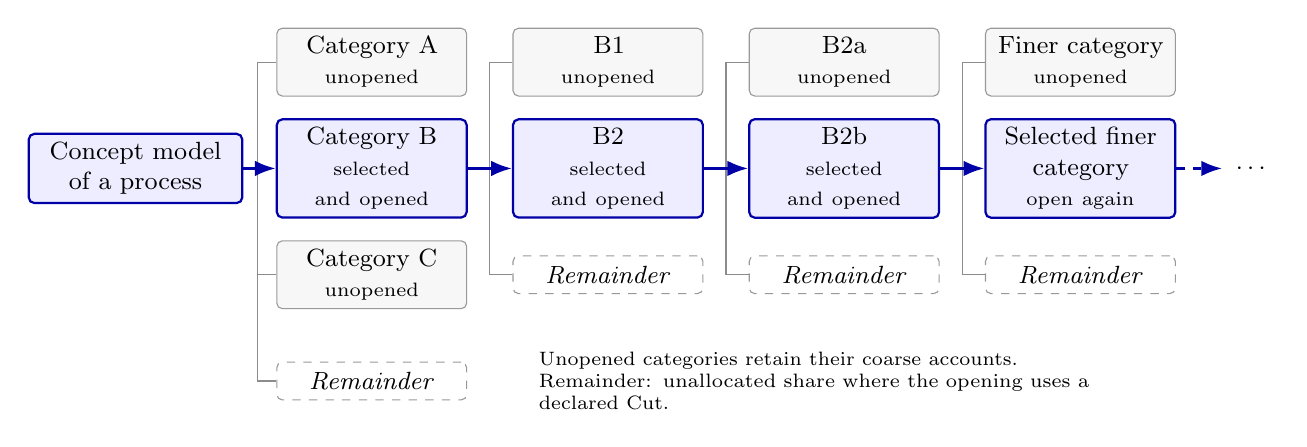
\begin{tikzpicture}[
  x=1cm,y=1cm,>=Latex,
  category/.style={draw=black!40,rounded corners=2pt,fill=black!3,
    align=center,font=\small,text width=2.2cm,minimum height=.76cm,
    inner sep=3pt},
  opened/.style={category,draw=blue!65!black,fill=blue!7,line width=.8pt},
  unopened/.style={category},
  remainder/.style={category,draw=black!40,dashed,fill=white,
    font=\small\itshape,minimum height=.48cm},
  branch/.style={draw=black!45,line width=.45pt},
  selected/.style={->,draw=blue!65!black,line width=1pt}
]
\node[opened,text width=2.5cm] (root) at (0,0)
  {Concept model\\of a process};

\node[unopened] (a) at (3,1.35) {Category A\\{\scriptsize unopened}};
\node[opened] (b) at (3,0) {Category B\\{\scriptsize selected and opened}};
\node[unopened] (c) at (3,-1.35) {Category C\\{\scriptsize unopened}};
\node[remainder] (r0) at (3,-2.7) {Remainder};

\node[unopened] (b1) at (6,1.35) {B1\\{\scriptsize unopened}};
\node[opened] (b2) at (6,0) {B2\\{\scriptsize selected and opened}};
\node[remainder] (r1) at (6,-1.35) {Remainder};

\node[unopened] (b2a) at (9,1.35) {B2a\\{\scriptsize unopened}};
\node[opened] (b2b) at (9,0) {B2b\\{\scriptsize selected and opened}};
\node[remainder] (r2) at (9,-1.35) {Remainder};

\node[unopened] (fine) at (12,1.35) {Finer category\\{\scriptsize unopened}};
\node[opened] (next) at (12,0) {Selected finer\\category\\{\scriptsize open again}};
\node[remainder] (r3) at (12,-1.35) {Remainder};

\draw[branch] (root.east) -- (1.55,0) |- (a.west);
\draw[branch] (1.55,0) |- (c.west);
\draw[branch] (1.55,0) |- (r0.west);
\draw[selected] (root.east) -- (b.west);

\draw[branch] (b.east) -- (4.5,0) |- (b1.west);
\draw[branch] (4.5,0) |- (r1.west);
\draw[selected] (b.east) -- (b2.west);

\draw[branch] (b2.east) -- (7.5,0) |- (b2a.west);
\draw[branch] (7.5,0) |- (r2.west);
\draw[selected] (b2.east) -- (b2b.west);

\draw[branch] (b2b.east) -- (10.5,0) |- (fine.west);
\draw[branch] (10.5,0) |- (r3.west);
\draw[selected] (b2b.east) -- (next.west);
\draw[selected,dashed] (next.east) -- (13.8,0);
\node[anchor=west,font=\small] at (13.85,0) {$\cdots$};

\node[anchor=west,align=left,font=\scriptsize,text width=7.5cm]
  at (5,-2.7) {Unopened categories retain their coarse accounts.\\
    Remainder: unallocated share where the opening uses a declared Cut.};
\end{tikzpicture}
\caption{Recursive conceptual decomposition of a process. Finer categories and
their relationships explain the selected parent; further openings deepen that
explanation. Selecting B, then B2, then B2b exposes finer categories while their
siblings remain at their existing resolution. The levels show conceptual depth, not successive periods;
the final arrow indicates that opening can continue. Blue marks the selected
branch. This is a selected view, not a requirement to construct a complete tree.}
\label{fig:conceptual-decomposition}
\end{figure}


\begin{samepage}
For example, someone requests and receives help. The people are Things; the
interaction is an Event whose Bindings state their roles. Helping is a Concept.
A process-based concept model describes the request, consent, action, and
consequences through the same forms, under its own declared model context.
A \emph{define} Realization links the Concept to that model; a \emph{describe}
Realization records the claim that this interaction instantiates it, with the
grounding version and role alignment. If graded fit is useful, a Cut on a
separate assessment Event carries the judgment. An UnderstandingNode explains
why it fits or why the definition needs revision. All six world forms can thus
participate; the explanation belongs to the understanding surface. The same
modeling language can therefore represent both a situation and a definition
used to interpret it.

\end{samepage}

An operational layer may add a recognizer that proposes a \emph{describe}
Realization and any component or aggregate fit Cuts from a world fragment, or
an instantiator that proposes a fragment from desired realization conditions.
Both retain their version and provenance and use the ordinary realization or
candidate-commit interface. Their omission from a construction is a profile
choice, not a restriction of the theory. This links the construction of an
example, the explanation of its concept membership, and the revision of that
concept through one representational medium. Learning those operators is a
further task, not a consequence of making their inputs explicit.

A concept-model family may retain context-specific models, counterexamples,
boundary cases, and unresolved variation. Numerical typicality uses a local Cut.

Define Realizations and typed links associate a concept with these resources.
A describe Realization records the comparison actually used: exemplars
consulted, or an alignment to a selected concept model. When graded fit is
required, separate component and aggregate fit Cuts sit under the relevant
assessment Events. The comparison is never implicit.

Examples do not uniquely determine new applications. A concept-model family adds
relational and temporal commitments; a recognizer adds a learned decision rule.
Either may remain incomplete or culturally local. Moving between them is a
possible learning path, not proof of a uniquely correct concept.

If the understanding process that authors or assesses a definition allocates
attention or responsibility across a concept model's components, a definition
or assessment Event about the model parents that Cut beneath the process.
This authoring or assessment process is distinct from the processes represented
within the concept model. Normalization applies only when its answers are mutually
exclusive shares of one named unit. Overlapping senses or perspectives remain
typed concept relations or separate Event-parented Cuts. The existence of
concept models does not by itself supply an operator by which their world
fragments recompose.

\subsection{Content-addressed grounding versions}

A Concept identifier and a grounding version answer different identity
questions. The identifier preserves the proposed concept across revisions. A
grounding version identifies the exact definition bundle used for one
Realization. A flat bundle may contain the identifier, description, relations,
prototype or exemplar references, and constraints; a deep bundle may contain a
process-based concept model and comparator specification. Either kind may be serialized
under a declared deterministic serialization scheme and addressed by its full Sema content hash
\cite{westerbergSema2026}. A revision produces another hash and an explicit
\texttt{supersedes} link. The Concept identifier remains only when its declared
continuity policy treats the revision as the same concept; a semantic split or
merger normally introduces linked successor identifiers.

Content identity is narrower than semantic identity. Equal digests under one
canonicalization scheme establish that two parties resolved the same serialized
representation;
they do not establish that differently encoded models have different meanings,
that the selected model is true, or that two perspectives accept its interpretation.
Human-readable shortened handles are therefore references, not the
authoritative identity. The full digest and canonicalization version remain in
the record.

Reproducible fit Cuts require the hashed or transitively addressed bundle to
name everything that can change the comparison. For a flat grounding this
includes its descriptions, relations, anchors, and constraints. For a process-based
concept model it additionally includes the fragment, role schema, component and
aggregate Cut questions with their answers and remainder, referenced grounding
versions, and comparator or recognizer version. A \emph{describe} Realization
then states exactly which bundle it used. Sema
provides addressing and agreement on that bundle; the Meaning Model continues
to carry context ancestry, evidence, alignment, and the claim made with it.

\subsection{A model of concept history}

The idealized fragment used to define a concept is not automatically an event
in the history of a modeled society. When the development of the concept itself
matters, the same grammar can instead model its historical carriers. A
formulation, notation, published definition, or versioned grounding bundle is
registered as a representational-token Thing linked to its Concept and
grounding hash. Its lifecycle and joint Events can then record formulation,
naming, publication, adoption, contestation, revision, or abandonment, with
people, documents, and institutions bound in their respective roles. A split or
merger of definition artifacts is recorded at this level; when the asserted
meaning itself divides or combines, linked successor Concept identifiers make
that semantic claim explicit. The Concept record remains a Concept; it is not
silently converted into a Thing.

This evidence-indexed subgraph records a \emph{concept history}. The wider
\emph{concept world} is the selected subgraph of Concept records, grounding
resources, typed relations, and histories, linked to instances through
Realizations. It groups records without granting shared authority or requiring
one universal ontology. Realizations connect it to ordinary world episodes, including cases
that exhibit a pattern before anyone names it. An insight Event may create a
new formulation or grounding version without claiming that it created every
possible meaning of the concept. A content-addressed registry preserves the
definition versions; the Meaning Model preserves the historical Events and
their disputed attribution. The first construction should open only the few
concept histories that materially affect its action.

Intellectual descent can also be attributed explicitly. A historian may ask
how a new mechanism drew on an earlier published method and a later discussion.
An assessment Event beneath the historian's perspective process can parent a
cause Cut allocating explanatory responsibility among the earlier publication
and discussion Events, linked to the predecessor Concepts and grounding
versions. Shared influences require a declared allocation convention or a joint
answer, with unresolved responsibility retained in the remainder. The
assessment retains its evidence cutoff; an UnderstandingNode explains the
attribution. Grounding hashes and supersession links do not by themselves
establish causal influence.

That social history differs from the reasoning by which someone defines or
interprets a concept. The latter is a Concept-scoped projection of the
Understanding Graph beneath a named understanding-process root and its clock.
It gathers nodes addressing the Concept identifier, exact grounding versions
or \emph{define} Realizations, evidence, rejected alternatives, and reasons for
retaining or superseding a grounding. An author's definitional history
normally unfolds in construction time; incompatible reasoning histories may
coexist without becoming accepted world state.

Preserving that reasoning requires a rationale UnderstandingNode for each
substantive initial freeze and committed revision, addressing the new grounding,
its predecessor if any, evidence, and material rejected alternatives. Without this
lineage the Concept remains valid but its rationale is not preserved. Simple
label registration and mechanical metadata changes need no ceremonial nodes.

The Book supplies a concrete starting point. In E20a, Lovelace identifies two
checking paths that share a prior value, and Babbage narrows his design's claim
from verification to internal comparison. Opening a concept history would
register the successive design formulations and link the revision to their
Concept and grounding versions. The later unscored model of a valid computational
claim makes independent comparison explicit; author note U14 explains the
episode. That note is not the character's own reasoning record, and these
materials do not yet constitute a versioned concept-history implementation.

\subsection{A process-based concept model: love and the Engine}

Consider an illustrative process-based concept model of devotional love of a
work, selected here as the canonical reference for a comparison. An
experiencer Thing and a work Thing participate in a process with an undertaking,
a response to difficulty, and continued engagement or preservation. These are
linked Events, not numerical shares of a life. Appraisals and wants belong
under the experiencer's inner-process root; the entire fragment has a declared
concept-model context.

A proposed alignment maps the experiencer to the Book's Babbage and the work
to his Analytical Engine project, distinct from the bounded apparatus and
calculation office. E06 supplies the finite undertaking; E25--26 supply a
setback and defensive response; E28--29 supply a changed interpretation and
preservation of the complete record. Attachment can be examined through
persistence, care through correction, desire through sought continuations, and
sacrifice through relinquished resources or control. These are overlapping
readings, not exclusive periods. This is an illustrative interpretation, not an
accepted love assessment or a claim about the historical Babbage.

Suppose a definition Event (the Event recording the definition) beneath one named understanding process carries a
Cut allocating one comparison budget among components $j$, with shares
$\alpha_j$ and remainder $\alpha_{\bot}$. Each component specifies a frozen,
weighted set of requirement checks. An assessment Event beneath that process
and about the target--component alignment carries a Cut dividing its local
check mass into \emph{matches}, \emph{does not match}, and unresolved remainder,
with shares $m_j$, $n_j$, and $u_j$. A recorded alignment $a$ may then derive
an aggregate fit Cut on the overall assessment Event:

\begin{equation}
  r_C=\sum_j\alpha_jm_j,\qquad
  n_C=\sum_j\alpha_jn_j,\qquad
  u_C=\alpha_{\bot}+\sum_j\alpha_ju_j,
  \qquad r_C+n_C+u_C=1,
  \label{eq:concept-match-theory}
\end{equation}

where $m_j+n_j+u_j=1$ in every component Cut. This is one possible comparator
for one grounding strategy, not a universal law of concepts. Its numbers are
all sibling-relative Cut shares; the Realization link itself remains unweighted.
The inputs are stipulated, not recovered from the Book.
They divide a comparison budget, not emotional intensity or
confidence that the episode occurred.
Here, the four named component Cuts each set
$u_j=0$; the aggregate $.100$ remainder comes entirely from the selected
model's unspecified component mass.

For a concrete stipulated care budget, assign $.50$ to retaining failed results
alongside successes, $.40$ to passing the complete record to a successor, and
$.10$ to immediately recognizing human checking as part of the work.
Let E28--29 satisfy the first two checks and Babbage's initial distancing in
E26 fail the third. Matched check mass is $.90$, unmatched mass $.10$, and
unresolved mass zero. These checks, weights, and judgments are illustrative,
not recovered Book assessments.

\begin{table}[H]
\centering
\small
\begin{tabular}{lrrrr}
\toprule
Reference component & $\alpha_j$ & $m_j$ & matches & does not match \\
\midrule
Care & .35 & .90 & .315 & .035 \\
Attachment & .25 & 1.00 & .250 & .000 \\
Desire & .15 & .60 & .090 & .060 \\
Sacrifice & .15 & .30 & .045 & .105 \\
Unspecified remainder & .10 & --- & --- & --- \\
\midrule
Aggregate fit Cut & & & $.700$ & $.200$ \\
Aggregate remainder & & & \multicolumn{2}{c}{$.100$} \\
\bottomrule
\end{tabular}
\caption{One inspectable fit Cut against a love model selected as a canonical reference.}
\label{tab:theory-love}
\end{table}

The useful result is not only the $.700/.200/.100$ aggregate Cut. It is the
recorded claim of strong fit on care and attachment, weaker fit on sacrifice,
and an alignment that treats a work as the object role. Another perspective may reject the alignment, select
a different love model, use exemplars instead, or decline to score the concept
without changing the target world.

Evaluative terms use the same plural grounding mechanism. A decision episode
may realize the model of situated intelligence or kindness reached through one
understanding process, and an assessment Event beneath that process may carry a fit Cut whose evidence and
grounding version remain inspectable. Later outcomes are separate Events, so an organized failure need
not be reclassified as an unintelligent action merely because it failed. A
coarse statement about a whole person remains perspective-scoped testimony or a
declared aggregation over episodes, never an intrinsic trait scalar. The grounding
may also declare thresholds or vetoes rather than assuming that all components
compensate linearly.

Constructing and revising these concept models uses the Meaning Model; learning
them and testing their empirical validity and transfer belong to Life
Simulation. Its ``Comparison frames for evaluative concepts'' subsection
proposes comparisons against a grounding, within one person's history, and
against matched reference episodes. Evaluator perspectives remain explicit,
and decision-time judgments stay separate from retrospective judgments
\cite{westerbergLifeSimulation2026}.

\subsection{Fit cuts and concurrent concepts}

One Event can be linked to both quarrel and farewell. If graded judgments are
useful, one assessment Event beneath the relevant perspective root for each Concept link carries
its own local fit Cut rather than making the Concepts siblings: quarrel might
have matches $.80$, does not match $.15$, and remainder $.05$, while
farewell has its own three shares. The two
match weights need not sum with each other because they belong to different
Cuts; within each Cut the three siblings do sum to one.

Fit and confidence ask different questions. A fragment may strongly exhibit a
concept while the evidence that the fragment occurred is weak; a well-attested
fragment may clearly fail to exhibit it. The fit Cut divides the declared
comparison unit into matched, unmatched, and unresolved portions. If numerical
confidence is needed, a separate epistemic assessment Event asks how support
divides among the claim, its rejection, and unresolved alternatives, with its
own anchors and evidence. It is not obtained as one minus non-fit, and the fit
remainder is not a universal uncertainty score. A construction may instead
leave confidence unquantified and mark the fit provisional or unscored.
Confidence weights neither multiply nor replace fit weights; a well-supported
mismatch remains different from a poorly supported match.

An emotion facet Cut supplies composition, not an absolute intensity scale. If
activation is assessed numerically, the divided unit must be explicit. One
option is a weighted set of checks for a declared ``materially active''
criterion: a separate assessment Event parents a Cut over matched, unmatched,
and unresolved check mass. A matched share of $.70$ means that checks carrying
$.70$ of this budget are satisfied, not that the emotion has intensity $.70$.
Activation can instead remain categorical and intensity unquantified.
Compatible fit or facet Cuts may be mixed across disjoint temporal children
under a stated question and aggregation. Occurrence is derived from Event
records.

\subsection{One World, Many Cuts}

The same accepted event can participate in several decompositions without
being copied. Consider Earth as a Thing and its modeled history as the bound
lifecycle Event over a geological horizon. Thing-side views may open Earth into
regions, the biosphere into ecosystems and organisms, or a person into body
systems. Event views may link overlapping geological, climatic, evolutionary,
and cultural processes, while a sequential Cut may partition the same history
into disjoint eras and transitions. One evening of reading can be reached
through at least two routes:

\begin{center}
\small
Earth history $\rightarrow$ evolution $\rightarrow$ human life
$\rightarrow$ one evening $\rightarrow$ reading,\\
Earth history $\rightarrow$ human culture $\rightarrow$ literature
$\rightarrow$ book production and circulation $\rightarrow$ reader encounter.
\end{center}

These are conceptual routes, not chains of normalized Cuts. Their arrows can
traverse different process, participation, and concept relations. A sequential
Cut divides History into disjoint eras by duration; a link from an episode to
its literary concept does not divide that unit. The reading Event still binds
the same reader, book, and place Things across these views.
Depending on the inquiry, that event can be opened through retinal activity,
emotional appraisal, cultural transmission, or narrative interpretation while
retaining its shared participants and source references.

An avalanche shows why direction cannot be a synonym for intention. A
snowpack, slope, terrain regions, and material layers are Things; the avalanche
is an Event bound to them. Physical-part events may expose slabs, layers,
cells, or particles. A sequential Cut may expose accumulation, instability,
trigger, fracture, release, runout, and deposition only at a lens where those
phases are ordered and disjoint. Loading, cohesion, friction, temperature,
velocity, terrain interaction, and entrainment are linked processes or
externally grounded physical data unless a separate question declares a unit
over mutually exclusive answers. At low
resolution an aggregate stability state and runout envelope may suffice. At a
finer resolution, local processes bind exposed material Things. Its direction
is physical: forces, constraints, and present state shape possible
continuations. Intentional language may be a useful metaphor, but the event
ancestry and direction type must not convert it into a claim about a mind.

\subsection{Direction from Tendency to Want}

For agent modeling, motivation can specialize direction without requiring an
unrelated primitive:

\begin{equation}
 \text{physical tendency}\quad\longrightarrow\quad
 \text{biological regulation}\quad\longrightarrow\quad
 \text{represented want}.
 \label{eq:direction-types}
\end{equation}

The arrow marks increasing representational commitments, not a claim that
every process secretly has a mind. A physical tendency follows forces and
constraints. Regulation detects or counteracts departure from a viability
region. A represented want exists when an actor represents or values a
possible state and that representation can alter action selection. Saying that
an avalanche ``wants'' to descend may compress an explanation; it remains an
instrumental description unless an internal representation is supported.

In this grammar, a want can be represented as an inner Event contained beneath
the relevant actor's lifecycle and inner-process root during a stretch of that
lifecycle. A construction may link it to a desired
condition of a registered Thing, Event, process, categorical state, or measured
world datum. It may then open the want into formation, activation, pursuit,
satisfaction, frustration, abandonment, or transformation. A plan is a
proposed continuation, and a decision commits one continuation under the
actor's represented beliefs, constraints, and competing wants. These are
profile choices with precedents in BDI and goal-systems research
\cite{raoGeorgeff1995,kruglanski2002}; the grammar preserves containment
ancestry, interval, question, and evidence without imposing one universal person decomposition or
one utility scalar.

Dramatic tension can also be modeled as an evolving process. Two characters
may depend on the same scarce resource; promises, deadlines, and discoveries
change their expectations, options, and relationship. A construction can open
this tension across the whole story, individual encounters, and momentary
choices, tracing how it builds, changes form, or resolves. These are linked
processes; any numerical Cut still names its question, divided unit, and
alternatives. Suspense attributed
to a reader is a separate process that unfolds as information is revealed.
It need not rise and fall with the conflict in story time.

\section{World, Understanding, and Artifacts}
\label{sec:interop}

The addressed construction supports three linked surfaces. The world surface
uses the six record forms. The understanding surface uses text-bearing
UnderstandingNodes from the Understanding Graph
\cite{westerbergUnderstanding2026}. The document surface holds text and code
artifacts as DocumentNodes.
They occupy one identifier space so that a question, reason, or sentence can
address the exact world record it concerns, but they retain different
semantics, clocks, and authority.

\begin{center}
\small\ttfamily
\begin{tabular}{@{}l@{}}
UnderstandingNode \{ id, type, text, created at, typed parents,\\
\qquad typed links, provenance \}\\
DocumentNode \{ id, role, text, discourse position, typed parents,\\
\qquad typed links, optional narrator and viewpoint metadata, provenance \}
\end{tabular}
\end{center}

These are surface records rather than seventh and eighth world forms. Every
UnderstandingNode has a typed containment path to a named
understanding-process root. Every DocumentNode has one to a named document
root; \texttt{story\_passage} is one DocumentNode role rather than a separate
record form. An UnderstandingNode externalizes a question, hypothesis,
prediction, tension, surprise, interpretation, reason, criticism, or revision,
among the node types of the Understanding Graph, and need not have an Event
interval or simplex. Kinds can be specialized to the application
without changing these parent-path obligations. A DocumentNode may hold a
report paragraph or code unit, as well as record an act of telling in discourse
order; document \emph{contains} and \emph{next} links do not inherit
Event-containment semantics.

Understanding links include \texttt{about}, \texttt{supports},
\texttt{contradicts}, \texttt{refines}, \texttt{answers},
\texttt{learned-from}, and \texttt{supersedes}. A DocumentNode links to Events
through \texttt{renders} and to an UnderstandingNode through \texttt{shaped-by}.
These links retain their surface-specific roles, not authority over their targets.
The implementation writes these names with underscores, for example
\texttt{learned\_from}. The original released Book import records its rendering
links as \texttt{expresses}; the later MCP passage workflow uses explicit
\texttt{renders} links to Events.

For example, a software investigation could link a measured response-time
history to a bottleneck hypothesis, the code unit changed to test it, and an
evaluation of the next measurement. The modeler can open a slow interval into
requests and their phases, or refine a bottleneck concept model to distinguish
causes requiring different tests. The result can change the explanation, the
code, or both.
This uses the same linked surfaces as the story examples below.

World authority is likewise topological. Every accepted world Event has a typed
containment path to History. A belief, appraisal, want, or estimate that is
itself part of the accepted world sits in a named inner Event process beneath
the relevant person's lifecycle. Its \texttt{about} links identify what is
believed or estimated without promoting that target claim to accepted world
state. A joint Event instead represents its participants through Bindings; it
does not acquire one participant's perspective merely by binding that
participant.

An imagined, remembered, or counterfactual scene has a named model-context
Event with a declared modality and source links. Accepting that Ada imagined a
successful trial accepts the imagining act, not the trial. The content's
depicted interval need not lie within the interval during which she imagined
it: context parenthood is distinct from temporal occurrence. A remembered
scene and an accepted historical account may address the same Things while
disagreeing about what happened. Promoting content into accepted world state
requires an explicit accepted assertion, not a traversal through its source.

An Event may carry an optional textual description. That field describes the
Event within its own record and ancestry; it is neither an UnderstandingNode
nor a DocumentNode. If a description must participate in a reasoning history
or in document order, a separate node is created under the applicable root and
linked to the Event. Text about an Event is not thereby that Event.

Optional narrator and viewpoint metadata refine a document role without
replacing its root path. Conflicting accounts can coexist across these
surfaces; agreement or common ground requires a declared derivation and is not
silently promoted to truth.

The density of the understanding surface is optional and explicit. A
construction may preserve no UnderstandingNodes, only rationales for consequential commitments and
revisions, or a finely segmented chronological reasoning trace. Absence means
``not externalized at this resolution,'' not ``no thought occurred.'' A dense
trace provides more supervision and auditability, but is not required for a
valid world. A claimed rationale trace declares which commitments require
nodes and which links connect their explanations. Conversely, an UnderstandingNode never gains world authority
merely because it is detailed. When its physical carrier matters, a stored note
or document is a representational-token Thing and its creation, reading,
transport, and revision are ordinary Events; its textual content remains on the
appropriate understanding or document surface.

The Concept-scoped projection described above uses this same understanding
surface. UnderstandingNodes carry reasons; Cuts carry numerical commitments.
A non-obvious Cut may link to its rationale node, which addresses the exact
Cut component or Event it explains.

Authorship may be performed by a human writer or a delegated agent. The human
who commissions and is responsible for the work is distinct from a modeled
fictional author persona, which is a represented person, not a role: the
persona's life may inform the work without making it the actual generator,
narrator, or character viewpoint.

An optional account may also represent the modeler as a Thing
with a declared identity, continuity criterion, lifecycle, and inner-process
root in the reading or construction context and clock, not the story's History.
Its changing attention, uncertainty, concern, and intentions can then be Event-processes.
UnderstandingNodes under its understanding-process root record its thoughts
about the world, concepts, or itself. Character-owned roots can likewise carry
thoughts about concepts; the subject does not determine whose thought it is.

For either a character or a modeler, inner activity may be recorded as
Event-processes, as UnderstandingNodes, through both, or not at all; the
construction chooses which form to use and where to open more detail. A node
can record a reaction beside the world Event, concept model, or passage it
addresses without a detailed process account, and a process account need not
include a dense thought trace. A derived view can collect such reactions under
their declared clocks and source references without adding new claims.
Inferring how concern changed between reactions is a further modeling step whose
process account retains its attribution and evidence; it can be constructed
directly or developed from the nodes, and neither form is a compulsory
replacement for the other.

World processes, concept models, and modeler processes name what records
describe, not new record forms. All can represent abstract content. This
optional account does not establish access to hidden cognition or neural
computation. The Reader of the Entangled Alignment proposal
\cite{westerbergEntangled2026} is one specific modeler role;
the general account also covers world construction, writing, and problem solving.

\subsection{Operative models and estimates}

An actor projection contains inner records active at a given time and accepted
records disclosed to the actor by then. Its inner records descend through that
actor's lifecycle and inner-process root; hypothetical targets remain within
that context. The subset organizing a decision is the actor's operative model.
Generation of speech or action
from that model is restricted to content actually recorded as observed,
communications received by the cutoff, and earlier records on the same
admissible paths. Co-presence permits an observation; it does not reveal every
field of an Event or another participant's private state. Observation and
delivery records therefore identify the content disclosed. Permission-aware
ancestry traversal cannot be used to bypass that boundary. A
contradiction with accepted History is therefore representable as
misperception rather than being silently repaired with author knowledge.
The same grammar can elaborate this projection into an attributed model of the
character's self, other people, and world, with distinct model contexts for
imagined or mistaken content. This is representational support, not a claim
that the Book already constructs those accounts in full.

An observer's account of the actor is different. It is an estimate Event beneath
the observer's inner-process root, linked \texttt{about} the target record, and
supported only by evidence accessible along that observer's paths. Self-report,
another character's estimate, an author's construction-time interpretation,
and the actor's operative state may all disagree. Compatible Cut estimates can
be compared by total variation and categorical claims by equality; those
divergences are derived diagnostics, not new semantic numbers. The profile also
bounds higher-order nesting---what one character thinks another thinks---rather
than granting unbounded omniscience. Life Simulation may later evaluate or
learn such estimates; their ancestry and access semantics belong to the Meaning
Model. A categorical, unit-bearing, or protocol-valued estimate retains the
target's data type and applicable unit or measurement protocol, with uncertainty
where relevant; an estimate of semantic composition uses a compatible Cut on the
estimate Event. Missing records or unequal coverage indicate ignorance or
noncoverage, not automatically disagreement or error.

\subsection{Transactional construction, rendering, and read-back}
\label{sec:construction-protocol}

World records, UnderstandingNodes, and DocumentNodes share one commit discipline.
The accepted parent is frozen. A proposal is a whole candidate delta containing
every new or superseding record required across the three surfaces. Validators
inspect it against that parent, including every new typed root path. In the
proposed workflow, the author or a designated checker decides whether to accept
a validated candidate. Rejection leaves the active graph unchanged, although a
construction log may retain the candidate and its explanation. Acceptance commits
the candidate atomically. A later change requires a new candidate, explicit
\texttt{supersedes} links, and revalidation of the affected dependency closure.
Current review records do not authenticate the reviewer, and not every
acceptance path requires a review record.

The commit envelope names the base snapshot and branch, candidate records and
links, replacement map, exact revisions read, applicable validators and
tolerances, and any refinement witness with its protected queries. This is
transaction metadata, not another world form. Each branch has one active
revision per logical identity. A stale base or changed read dependency rejects
the candidate; rebasing requires renewed validation. Matching identifiers do
not merge branches. Commit appends one immutable cross-surface snapshot and
advances its head atomically.

Revision preserves predecessor records and revalidates affected dependents.
Operators, including opaque ones, must declare the records they read; source-bound
views and passages also record derivation dependencies. Those declared links
determine which dependents must be rechecked, regenerated, or marked stale.
A generic \texttt{about} link alone does not define such a dependency. These
are the required semantics; the current Rust host does not implement every
cross-surface step.

The Introduction's illustrative trial now has a record-level reading. Its
Event, grounding Realization, assessment Cut, rationale UnderstandingNode, and
rendered DocumentNode address exact revisions. A changed success claim enters
as one candidate containing the affected records, with declared dependents
rechecked or marked stale. Co-storage alone does not establish their agreement;
the acceptance checks and semantic judgment do that work.

A direction Cut can make the generator's freedom inspectable. Its children are
mutually exclusive candidate continuations and its remainder retains options
not articulated. A draw that selects the remainder requires a new admissible
proposal; it must not silently discard that mass and renormalize the named
answers. The constructor may fix mass needed by the premise or an
earlier commitment, draw among the remaining alternatives with a recorded seed,
and then build the selected continuation as a complete candidate. A poor draw
may be rejected under preregistered gates, but it is not silently rerolled until
the author likes the answer. Rejected siblings and reasons remain addressable.
Thus the model can materially decide the story while authorship remains bounded
by declared constraints and visible intervention.

A rendering route records the source commit and epistemic status; an ordered
route through Events and its currently opened frontier; optional narrator and
viewpoint metadata; the evidence accessible at its declared cutoff; a
disclosure policy; and the target DocumentNode with role
\texttt{story\_passage}. It specifies which evidence the renderer may use
under the chosen viewpoint and disclosure policy. In character-limited
narration, this excludes later facts, private state unavailable to that
character, and undelivered documents. Other narrative viewpoints obey their
declared access and disclosure rules. Enforcement and read-back must check that
the generated prose respects those limits. The route is a construction profile over existing
references, not a seventh world relation.

Read-back applies the inverse operation in a fresh context: infer the Things,
Events, Bindings, Cuts, Realizations, typed ancestry, and links implied by a story-passage
DocumentNode, then compare that proposal with the source commit. A mismatch can
expose an omitted record, an unsupported sentence, a wrong root path, or prose
that implies a different composition. Its resolution is another explicit
candidate: revise the DocumentNode, revise the model with justification, or
retain a declared ambiguity. A read-back UnderstandingNode under the named
review process preserves the disagreement and decision. This closes the loop
from model to prose and back without treating prose as the sole authoritative
copy.

Readers track situations and update their accounts when perceived event
boundaries disrupt expectations \cite{zacksEtAl2007event,zwaanRadvansky1998}.
Read-back asks where such an update no longer follows the intended route;
the reader's interpretation remains distinct from the modeled interior and
the author's reason.

\subsection{The unfunded successor, 1852--54}

Chapter X of the completed \emph{Book of Conditions}, \emph{The Unfunded
Successor}, supplies an actual construction example. At Ockham in August
1852, Lovelace recognizes that both her claim authority and Neale's independent
checking depend on single people. She asks for funded training and outside
supervision of a second checker. Babbage brings a mechanical self-comparison
design, then recommends waiting; Halden defers the expenditure. Lovelace dies
with the request unanswered. In 1854 Halden authorizes delivery without the
independent check, and Guardian returns the erroneous table. These are the
finished Book's authored events and character interpretations, not evidence
about the historical minds of Babbage or Lovelace.

The construction's world descriptions identify the succession decision as
E20, Lovelace's death as E21, the omitted check as E24, and the returned table
as E25. Understanding note U05 explains why her death removes active pressure
but neither inserts the wrong number nor forces Halden's decision. Chapter X
renders the earlier succession episode; Chapter I opens with the later
failure. Figure~\ref{fig:book-succession} maps these existing materials onto the
three surfaces: character interpretations belong beneath their inner-process
roots, U05 supplies the construction-time rationale, and the chapters supply
DocumentNode text with role \texttt{story\_passage}. The notes and chapters were
subsequently imported as native surface records
(Section~\ref{sec:book-construction}). That retrospective receipt does not
recover the original cross-surface authoring transactions.

\begin{figure}[!htbp]
\centering
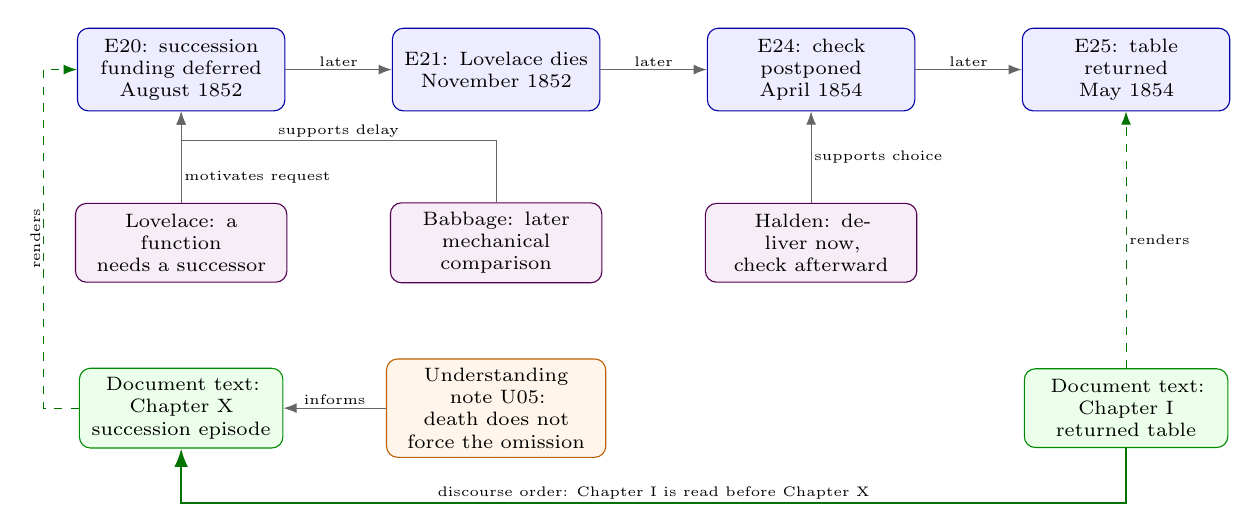
\begin{tikzpicture}[
  x=1cm,y=1cm,>=Latex,
  world/.style={draw=blue!65!black,rounded corners,fill=blue!7,align=center,
    font=\scriptsize,text width=2.4cm,minimum height=1.05cm},
  inner/.style={draw=violet!65!black,rounded corners,fill=violet!7,align=center,
    font=\scriptsize,text width=2.45cm,minimum height=1cm},
  author/.style={draw=orange!75!black,rounded corners,fill=orange!8,align=center,
    font=\scriptsize,text width=2.55cm,minimum height=1cm},
  render/.style={draw=green!55!black,rounded corners,fill=green!8,align=center,
    font=\scriptsize,text width=2.35cm,minimum height=1cm},
  edge/.style={->,thin,draw=black!60},
  label/.style={font=\tiny,fill=white,inner sep=1pt}
]
\node[world] (request) at (0,2.7) {E20: succession\\funding deferred\\August 1852};
\node[world] (death) at (4,2.7) {E21: Lovelace dies\\November 1852};
\node[world] (omit) at (8,2.7) {E24: check postponed\\April 1854};
\node[world] (return) at (12,2.7) {E25: table returned\\May 1854};
\node[inner] (ada) at (0,.5) {Lovelace: a function\\needs a successor};
\node[inner] (babbage) at (4,.5) {Babbage: later\\mechanical comparison};
\node[inner] (halden) at (8,.5) {Halden: deliver now,\\check afterward};
\node[render] (chapterX) at (0,-1.6) {Document text:\\Chapter X\\succession episode};
\node[author] (note) at (4,-1.6) {Understanding note U05:\\death does not\\force the omission};
\node[render] (chapterI) at (12,-1.6) {Document text:\\Chapter I\\returned table};
\draw[edge] (request) -- node[label,above]{later} (death);
\draw[edge] (death) -- node[label,above]{later} (omit);
\draw[edge] (omit) -- node[label,above]{later} (return);
\draw[edge] (ada) -- node[label,pos=.28,right]{motivates request} (request);
\draw[edge] (babbage.north) -- (4,1.8) --
  node[label,above]{supports delay} (0,1.8) -- (request.south);
\draw[edge] (halden) -- node[label,right]{supports choice} (omit);
\draw[edge] (note) -- node[label,above]{informs} (chapterX);
\draw[edge,dashed,draw=green!45!black] (chapterX.west) -- (-1.75,-1.6) --
  node[label,rotate=90,above]{renders} (-1.75,2.7) -- (request.west);
\draw[edge,dashed,draw=green!45!black] (chapterI) --
  node[label,right]{renders} (return);
\draw[edge,thick,draw=green!45!black] (chapterI.south) -- (12,-2.8) --
  node[label,above]{discourse order: Chapter I is read before Chapter X}
  (0,-2.8) -- (chapterX.south);
\end{tikzpicture}
\caption{Selected records from the completed Book, mapped to world,
understanding, and document surfaces. The top arrows show story order, not
causal necessity. U05 belongs to construction time; the bottom arrow shows
the different order in which the reader encounters the events. Character
interpretations and the author's explanation remain distinct. Edge labels
are explanatory glosses, not literal Understanding Graph edge-type names.}
\label{fig:book-succession}
\end{figure}

\section{Closure and Sufficiency}
\label{sec:closure}

Closure is claimed only relative to a declared purpose and resolution. This
section first asks whether the same records can be refined recursively without
erasing accepted commitments, then turns that capacity into a finite-resolution
sufficiency test.

\subsection{Recursive refinement at a declared resolution}

Suppose a finite-resolution world contains the world records above. Opening
a thing adds things and events that preserve the parent's identity boundary.
Opening an Event may admit qualified child answers under a declared Cut, expose
concurrent Event-processes, add linked episodes and updating Events, or expose
typed world data. Only a Cut invokes a one-unit composition contract; a sequential Cut
additionally requires disjoint intervals and derived duration shares.
Describing a target adds a realization record using one declared concept
grounding. If that grounding is a process-based concept model, its role-bearing things and
events reuse the same world grammar. In this restricted sense, world-record
refinement is recursively closed.

The grammar places no intrinsic lower or upper bound on modeled resolution. A cell,
person, institution, planet, or galaxy uses the same Thing--lifecycle pairing
when its identity and persistence matter; organelles, group members, or stars
can be exposed through time-scoped relations; and biochemical changes,
decisions, discoveries, mergers, or explosions are Events at the resolution in
which they matter. Containment and temporal refinement provide hierarchical
views, while overlapping processes and cross-resolution update links keep the full
representation a graph rather than one tree. Domain content remains specific:
a cell may require biochemistry and a galaxy astrophysics, and neither acquires
an inner-process ancestry merely by sharing the grammar. Increasing model
capability may open unresolved remainder, propose and test better boundaries,
processes, unit-bearing world data, and candidate domain laws, and check compatibility across resolutions.
It need not merely add detail; a better abstraction may justify an explicit
revision that supersedes many weak records with a smaller, more predictive
account. This is a claim of representational extensibility,
not that the present model knows every resolution or that every process follows
jump diffusion.

As a long-term theoretical goal, the representation could support opening a
scene into molecular or particle-scale processes where the inquiry requires
them. Reactions and collisions are Events; tracked
entities can use Things with declared identity and continuity. Collective or
field descriptions need not assign a separate Thing to every constituent.
Attached physical or chemical models could compute their evolution, retaining
their units and approximations. The finer results must preserve the protected
coarse answers under declared mappings and tolerances, or prompt explicit
revision. What changes at these depths is the domain model and its evidence
standard, not the six record forms.

Psychological resolution follows the same rule. A person profile selects
questions for a construction, not the expressive limits of the grammar.
There is no prescribed maximum depth or universal personality tree. A coarse
account of an authored character's resistance to delegation might be opened
into concerns about accuracy and recognition, beliefs about a colleague's
competence, and memories of broken promises. Further detail could distinguish
private collaboration from public assessment, or trace how later experiences
alter that difference. These remain interpretations in the relevant actor or
observer context, not psychological facts established by adding detail.

A more capable model could choose different questions, boundaries, and depths
according to what a scene or inquiry needs to explain. Competing motives may
form a Cut under a declared attention question; beliefs, memories, and
relationship Events remain linked processes without being normalized together.
An opening under the same question must preserve its declared coarse
commitments. A different question creates another view, while a changed account
requires explicit revision. Thus psychological refinement can elaborate,
reorganize, or simplify a person's model rather than merely populate a fixed
template.

More capable systems, potentially including artificial superintelligence, may
extend this work to detail far beyond categories humans can readily understand.
Protected coarse queries can still expose a readable account of fatigue,
trust, or responsibility. Finer records must reconstruct those answers within
the declared tolerances or revise the commitments explicitly. A Cut's remainder
keeps unallocated share visible under its question. These contracts preserve
continuity; comparisons on unseen cases must test whether the unfamiliar
distinctions improve the account. Meaning Model supplies this representational freedom and its
preservation contracts; Life Simulation considers how to learn which
refinements are useful.

This is not a theorem that every true explanation is a weighted tree. Cuts may
cross; events can be both causes and consequences under different questions;
and domains can attach specialized measured data, laws, fields, or solvers.
Those attachments are content referenced by events. Nor does the claim imply that
cognitive testimony or prose must be encoded as cuts. The Understanding Graph
and document surface remain interoperating representations with different
jobs.

\subsection{Finite-resolution sufficiency as a test}

A representation is sufficient only relative to a query, tolerance, and cost.
For a story-coherence query, the identity of the Engine, the intervals of key
events, who held each belief, and how fine emotions recompose may be sufficient.
For stress analysis of a gear, the same representation must point to geometric
and physical state that this paper does not attempt to replace.

The bounded constructive argument is deliberately modest. Any finitely
specified simulator with computable or approximable transitions over a bounded
horizon can be wrapped in one root Thing and its lifecycle/root Event: place the
simulator configuration in event state, reference its transition semantics as
direction, and expose its outputs through typed observations. If nothing more
is known, leave the root opaque. Later useful identities and processes can be
opened through Things, joint Events, and cuts while the root behavior remains a
consistency check. Bare representational universality is therefore cheap. The
substantial hypothesis is that useful stable identities and cuts exist and
improve compression, prediction, explanation, control, or coherent generation
enough to justify their cost.

The sufficiency claim can fail in three ways. A required distinction may fit no
record profile. A composition rule may destroy information needed at a coarser
level. Or the cost of explicit articulation may exceed its value. Such failures
should produce a remainder when a governing Cut exists, leave other detail
implicit or add a domain attachment, or reject the grammar for that task--not
a declaration that the world has been fully represented.

Cross-cut identity is the main defense against false trees. Einstein can be
important in a scientific cut and nearly absent in another person's daily-life
cut without being duplicated. A relationship can participate in emotional,
economic, and legal cuts. Local weights answer local questions; the shared
thing and event identifiers preserve that these descriptions concern the same
world.

Five questions provide the evaluation contract:

\begin{enumerate}
  \item \textbf{Coverage:} Can the target be represented without changing the
    concept, Thing, Event, Binding, Cut, and Realization grammar?
  \item \textbf{Reference:} Do descriptions and roles resolve to the intended
    continuing Things across time and opened detail, while explicit split,
    merge, replacement, and succession events change identity when required?
  \item \textbf{Grounding:} Where a comparator or recognizer is declared, does it
    distinguish held-out instances from counterexamples under that grounding?
    Otherwise, do independent reviewers agree with
    the construction's applications to held-out instances and counterexamples
    under its declared grounding and context? Both checks retain unresolved
    cases. Calibration applies only to declared
    probabilistic outputs, not to fit shares of requirement-check mass.
  \item \textbf{Recomposition:} Do admitted children recover their parent's
    declared Cut commitments within the frozen tolerance, and do Event-process
    links, role bindings, identities, and typed world data satisfy their own
    contracts without being treated as Cut weights?
  \item \textbf{Value:} Does refinement improve prediction, explanation,
    control, or coherent generation enough to justify construction,
    validation, inference, and maintenance cost?
\end{enumerate}

\section{\emph{The Book of Conditions}: Completed Book, Partial Witness}
\label{sec:book-construction}

\emph{The Book of Conditions} is a completed twelve-chapter manuscript with
an authored world, selected concept grounding, rooted UnderstandingNodes, and
an ordered story route. The AI constructor built it under my direction at the beginning, while the tool
itself was being developed; later revisions were made by language-model agents
through the tool.
It is a partial construction witness, not a complete protocol implementation,
built anew from a released historical prefix and an explicit counterfactual divergence. No
discarded preliminary draft supplies evidence, accepted records, counts, or prose.
This tests whether the grammar can hold
one inspectable long story at a declared resolution; it does not demonstrate
every permitted profile or establish comparative advantage.

The Book is one continuing work. The construction history, import receipt,
and numerical portrait below report its initial construction;
Section~\ref{sec:story-continuations} follows its subsequent revisions and
describes the current model. Measurements and reviews remain attributed to
the revisions they examined.

\subsection{How the construction proceeded}

The original Book construction proceeded in six rounds.

\begin{enumerate}
  \item Preparation fixed the historical cutoff, premise, vocabularies, access
    rules, and budget. Preparation prose remained external, not runtime authority.
  \item The constructor registered roots, historical prefix, Things,
    lifecycles, relationship and presence Events, and thirty-four Concept
    bundles, retaining unresolved documentary detail.
  \item Five isolated whole-history candidates were generated under a common
    schema. All were rejected: negotiation lacked a credible route to priced,
    accountable construction. None was admitted to History by a Direction roll.
  \item A pragmatic successor was then written first as one paragraph and
    expanded successively to two, three, four, and five paragraphs. Opening the
    account exposed the missing commercial founder. Local defects prompted
    repairs, not restarts unless the parent history failed.
  \item Thirteen lifecycles and coarse life accounts were placed before three
    principals were opened into concurrent processes, local Cuts, and linked
    UnderstandingNodes. Events, relationships, ledgers, and one concept model
    elaborated or explicitly revised the macro account.
  \item Twelve route units were selected and rendered. Later literary passes
    report updating Event and life descriptions before corresponding prose;
    changes without new world facts remained rendering decisions.
\end{enumerate}

Saved checkpoints demonstrate coordinated revision, not every within-round
editing order or the fully automated transaction protocol. The final world was
not chosen by a preregistered Direction draw; missing logs cannot be recovered
retrospectively.

\subsection{A Book-specific profile}

From Universe and History, the construction registered the needed people,
institutions, places, documents, machine parts, and collective processes.
Lifecycles, relations, presence, and historical data established the prefix.
Character interiors sit beneath the person's lifecycle and inner-process root;
they are not facts about historical minds. Presence, communication, delivered
evidence, and typed ancestry limit each actor projection to what the character
could know at its cutoff.

For principals, the Book uses the compact profile in
Table~\ref{tab:book-person-profile}, which distinguishes accepted coverage from
deeper preparation choices.
Appendix~\ref{app:atomic-wants} explains the AtomicWant leaves and their
conditional attention units.

These categories are a first draft, not a finding. The intended practice is
iterative: humans and AI construct characters, compare which decompositions
produce coherent, distinctive behavior that depends on the numbers, and test
which distinctions can be recovered from the resulting text. They revise the
vocabulary between runs, including proposing categories that no current human
vocabulary names. Revised concept groundings receive new content hashes; each
run retains the versions it used, so earlier constructions remain readable.
The grammar supplies a reusable language while the categories improve through
this construction and testing cycle. Life Simulation develops the dependence
and recovery tests; the completed Book is a starting construction, not a
completed comparison of vocabularies.

\begin{table}[H]
\centering
\small
\begin{tabularx}{\textwidth}{@{}p{0.11\textwidth}Y@{}}
\toprule
View & First-construction reading \\
\midrule
IS & Nine concurrent, unweighted life processes: body, kin, partnership, work,
place, means, knowledge, standing, and meaning. They may overlap and do not sum. \\
WHAT & Accepted scene Cuts open concern. The preparation profile additionally
specifies conditional approach/threat-avoidance and AtomicWant Cuts; those
deeper numerical openings were not exercised. A distinct chain links an
avoidance want to a threat-belief Event, fear appraisal, and action. \\
HOW & Event-parented scene Cuts divide problem-solving attention among framing,
deciding, and remainder, with conditional concrete/abstract and
impartial/personal views. Strategies remain linked records unless another unit
justifies a Cut. \\
FEELS & A scene appraisal Event parents the emotion Cut. It is compared with
supported wants, beliefs, and Events rather than treated as a consequence of
the concern weights alone. \\
\bottomrule
\end{tabularx}
\caption{The Book's IS/WHAT/HOW/FEELS profile: accepted coverage and deeper preparation choices.}
\label{tab:book-person-profile}
\end{table}

The person template archived in the
\href{https://github.com/emergent-wisdom/meaning-model/blob/v0.5.2/examples/book-of-conditions/PERSON-TEMPLATE.md}{v0.5.2 example}
offers a different deeper opening: AtomicWant Cuts directly under concerns, with separate outlook Cuts. Accepted scene
records contain concern-level WHAT weights and qualitative want Events, not
either deeper numerical tree. The appendix preserves the preparation scheme
without treating it as a demonstrated construction result.

The Book's scene and coarse period profiles are authored. A finer temporal
opening must recompose its parent by duration and report coverage; the selected
scenes do not yet supply that complete partition. Conditional profiles reuse records under named
situations and participant sets. The selected concerns, strategies, emotions,
temporal resolutions, and person leaves are first-construction vocabulary, not
universal human structure. Every nested Cut has an Event parent beneath
the applicable inner process, names its conditional unit, and retains a tested
remainder.

The Book's derived shock profile applies Section~\ref{sec:multiscale-change}:
it names the affected processes, available prior expectations, response Events,
and descriptive adaptation shape. Table~\ref{tab:book-cross-scale-change}
locates the pattern in actual accepted records, from the historical setting
to opened trial phases. Success itself is consequential: shared pleasure at
E14 and subsequent inquiries at E16 reinforce the confidence behind E18's
overexpansion. Adaptation is therefore not always prudent adjustment.

\begin{table}[htbp]
\centering
\small
\begin{tabularx}{\textwidth}{@{}>{\raggedright\arraybackslash}p{0.19\textwidth}YY@{}}
\toprule
Resolution & Antecedent and perturbation & Recorded response \\
\midrule
Historical setting, 1847--48 & Staged finance supports manufacture; wider
credit contraction delays a subscription call (E11). & Existing wages are
paid, new work slows, and the undertaking does not enlarge its scope to
attract money. A coarse historical process constrains workshop activity. \\
Institution and lives, 1852--71 & Lovelace identifies the succession risk
(E20); her death ends her active role (E21). The later returned table exposes
the checking failure (E25). & Disclosure and correction (E26) precede office
closure (E27). Babbage's interpretation changes over years (E28), ending in
custody of the complete record, including failure (E29). \\
Project episode, July--November 1846 & Individually conforming assemblies
bind under a shared drive (E09). & Interface rework (E10) restores operation
at a cost in time and money while preserving the contracted apparatus,
rather than authorizing every proposed redesign. \\
Trial and its phases, May 1851 & A frozen test packet (E13) precedes the
clearing failure and stopped run (E14a). & The run is restarted; complete
agreement supports the bounded claim (E14b), followed by shared pleasure
(E14c). The prose opens the waiting and recognition further, card by card. \\
\bottomrule
\end{tabularx}
\caption{Cross-scale anticipation, perturbation, and response in the authored
Book. The rows are linked readings, not exclusive Cut children. The opened
trial phases have no exact minute durations or within-scene numerical curve.}
\label{tab:book-cross-scale-change}
\end{table}

These cases support representational coverage, not a universal cycle theory.
In particular, U05 separates the anticipated succession failure from the
transcription and delivery choices: Lovelace's death neither enters the wrong
number nor compels omission of the check. The longer arc is explained through
those intervening Events, not by treating one loss as sufficient cause.

The construction used a frozen flat Concept registry: identifiers,
one-line descriptions, obvious typed relations, and exemplar anchors only
where a judgment required them. Thirty-four bundles received content-addressed
grounding versions. Prototypes and process-based concept models were excluded from the
flat registry; after the world was accepted, one small model of a valid
computational claim was opened as an unscored integration example. The
love--Engine model in
Table~\ref{tab:theory-love} shows the intended arithmetic without prejudging
the Book's choice. Three concept histories at most were permitted where
invention or revision materially affected the story; all other histories
remained unopened.

Preparation specified a $.10$ elicitation grid with supported $.05$ refinement.
The accepted pragmatic successor instead retains directly authored decimal
shares, including $.76$ and $.72$ in scene-outlook Cuts. The retained record
does not document a grid amendment or establish compliance with that rule.
The retrospective import preserves those source weights and checks their sums;
no transformation from the earlier grid is claimed. Other selected limits were
no continuous extents, an estimate-depth cap of two, and full scene profiles
only for the three principals. These are construction choices, not grammar
obligations.

\subsection{Construction artifact, Rust host, and validation boundary}

The first construction's retrospective import recorded source digests, a
persisted Rust compilation response, 117 person-process addresses, 107 authored Cuts plus one derived
duration Cut, and linked document and understanding nodes in SQLite. Reloading
recovered that model; native document rendering reproduced that manuscript.
This was a retrospective import receipt, not a source-locked transaction for
the original construction or an independent read-back record.
That historical bundle remains in the
\href{https://github.com/emergent-wisdom/meaning-model/tree/v0.5.2/examples/book-of-conditions}{v0.5.2 repository history}.
The current bundle is identified separately below. The engine remains in
\texttt{rust-engine/}, with its MCP interface alongside it.

Sema minted and verified the thirty-four flat definition bundles so that each
has a content-addressed grounding version \cite{westerbergSema2026}. The Rust
host compiled forty structural authoring profiles: thirteen persons, nineteen
other Things, three relationships, one Concept, and four change arcs. These
loaders create openable scaffolds, not semantic scalars. Psychological numbers
remain Cut weights; pounds, hours, dates, and counts remain world data.

Table~\ref{tab:book-enforcement-boundary} states the implementation boundary.
The synthetic conformance suite of development checkpoint 06 passed all 31
positive and negative fixture expectations, seven report checks, and three
targeted Rust tests; that checkpoint is not included in this release. These are mechanism checks, not evidence that the authored history,
character interpretations, or prose are true or good.

\begin{table}[htbp]
\centering
\small
\begin{tabularx}{\textwidth}{@{}p{0.22\textwidth}YY@{}}
\toprule
Layer & Exercised in the construction & Not established \\
\midrule
Rust host & Profile compilation, immutable persistence, Cut normalization,
component addresses, nearest-root ancestry, and source-bound document rendering &
Complete mixture closure, cutoff-safe context assembly, independent read-back,
or recovery of the original authoring transactions \\
External validator & Cut sums and remainders, selected recomposition fixtures,
lifecycles, ancestry, presence, access, person-profile shape, and route
exclusions & Historical or psychological validity, cross-surface atomicity of
the final pragmatic successor, or independent prose recovery \\
Authored construction & Macro revision, Event and life descriptions, local Cut
judgments, UnderstandingNodes, route selection, and prose & Automatic induction,
forecast calibration, or an empirical advantage over unstructured writing \\
\bottomrule
\end{tabularx}
\caption{What the first construction exercised and what remains outside the
implementation claim.}
\label{tab:book-enforcement-boundary}
\end{table}

\subsection{Descriptive numerical portrait}

The numerical portrait uses three categories. Cut weights are represented
sibling-relative shares under one named question and remainder. Typed world
data retain external units. Counts, density, total variation, means, and ranges
are derived operational diagnostics rather than additional facts in the world.
Table~\ref{tab:book-footprint} reports the first construction at its declared
resolution; duplicate display tables are excluded from the Cut inventory.

\begin{table}[htbp]
\centering
\small
\begin{tabularx}{\textwidth}{@{}Y r@{}}
\toprule
Construction quantity & Count \\
\midrule
Flat content-addressed Concept bundles & 34 \\
Inventoried authored Cut instances & 107 \\
Child and remainder weights in those Cuts & 472 \\
Primary numbered Events plus explicitly opened child Events & $30+7$ \\
Complete human lifecycles at the declared resolution & 13 (3 detailed, 10 coarse) \\
Macro trajectories and named phases & 4 trajectories, 13 phases \\
Rendered chapters and manuscript words & 12 chapters, 11,046 words \\
Distinct Cuts per thousand rendered words & 9.69 \\
\bottomrule
\end{tabularx}
\caption{Descriptive footprint of the accepted first construction. Density is
a maintenance and representation statistic, not a quality score.}
\label{tab:book-footprint}
\end{table}

The 107 Cuts divide into 12 scene-WHAT, 13 scene-outlook, 27 scene-HOW, 9
scene-FEELS, 11 slow-outlook, 11 threat-character, 13 health, and 10 world
decision or forecast Cuts, plus one concept-model component allocation with zero
remainder. Among the eight earlier families, mean remainder ranges from .060 to .081;
the full observed range is .04 to .20. No global semantic mean is computed,
because the questions and divided units differ.

An outlook Cut divides one unit of represented outlook toward fulfillment of
active wants. Assurance means believing that a wanted endpoint remains
available or will be attained; threat means believing it may be obstructed or
lost. Babbage's May 1851 trial Cut assigns .76 to assurance, .18 to threat, and
.06 to unresolved outlook. Lovelace's assured share is .70 and Halden's .72.
These authored readings are not endpoint probabilities or emotional intensities.

The comparison differs from a world constraint. In February 1852, the local expansion
margin $w(\text{accept four})-w(\text{limit to two})$ is +.30, -.50, and +.20
respectively. These are not votes: Halden alone holds contracting authority.
The world-unit constraint is independent of those interpretations. In the
first construction, four jobs require $4\times40=160$ checker-hours against
80 protected hours, a twofold demand-to-capacity ratio and an 80-hour deficit.
The later allocation of preparation and final checking is described in
Section~\ref{sec:story-continuations}.

Nested opening remains local. Early Babbage's threatened-fulfillment share .64
multiplied by autonomy-at-risk .34 gives .2176 of that period's full outlook
unit because the second Cut explicitly opens the first; it is not a free fear
score. The separate whole-history partition has six disjoint periods, from
18 August 1843 to 19 October 1871. They cover 10,289 days exactly, so their sequential
shares sum to one by duration while saying nothing about narrative importance.
For compatible Cut vectors, total variation is half the sum of absolute
differences, including remainder: the minimum share that must move between
categories to turn one allocation into the other. It ranges from .11 to .31
across eight adjacent slow-outlook transitions and from .38 to .60 across four
selected scene transitions. This is a descriptive authored pattern, not a fitted
shock law or population result. The
\href{https://github.com/emergent-wisdom/meaning-model/blob/v0.5.2/examples/book-of-conditions/NUMERICAL-STATISTICS.md}{numerical supplement archived with v0.5.2}
retains the family, ledger, apparatus, and duration tables. None of these diagnostics establishes
predictive validity, population psychology, causal identification, or superiority
over an unstructured writing process.

Figures~\ref{fig:book-slow-outlook} and~\ref{fig:book-scene-simplex} make the
long and short views visible without inventing an absolute psychological
scale. The first plots compatible period Cuts as categorical intervals. The
second plots compatible scene Cuts inside their shared simplex. Neither is a
fitted temporal function: the marks display authored commitments at the
resolutions actually opened by the construction.
For example, Babbage's assured share is .79 at expansion, .28 at the returned
table, and .51 at custody. The last point accompanies a changed interpretation
of the work, not a return to expansion confidence. These are sibling-relative
authored appraisals, not forecast probabilities or a measured recovery curve.

% Descriptive figures derived from the accepted first-construction Cuts.
% These are authored compositions, not measurements of historical people.

\begin{figure}[htbp]
\centering
\begingroup
\colorlet{mmassured}{blue!62!black}
\colorlet{mmthreat}{orange!82!black}
\colorlet{mmremainder}{black!22}
\newcommand{\MMOutlookBar}[4]{%
  \pgfmathsetmacro{\mmright}{#1+0.58}%
  \pgfmathsetmacro{\mmtop}{#2+#3}%
  \fill[mmassured] (#1,0) rectangle (\mmright,#2);
  \fill[mmthreat] (#1,#2) rectangle (\mmright,\mmtop);
  \fill[mmremainder] (#1,\mmtop) rectangle (\mmright,1);
  \draw[black!45,thin] (#1,0) rectangle (\mmright,1);
  \node[font=\tiny,rotate=48,anchor=east] at ({#1+0.29},-0.035) {#4};
}
\begin{tikzpicture}[x=1cm,y=4.05cm]
  \fill[mmassured] (2.15,1.13) rectangle +(0.22,0.055);
  \node[font=\scriptsize,anchor=west] at (2.42,1.157) {assured};
  \fill[mmthreat] (4.20,1.13) rectangle +(0.22,0.055);
  \node[font=\scriptsize,anchor=west] at (4.47,1.157) {threatened};
  \fill[mmremainder] (6.85,1.13) rectangle +(0.22,0.055);
  \node[font=\scriptsize,anchor=west] at (7.12,1.157) {unresolved};

  \draw[black!55,->] (-0.15,0) -- (-0.15,1.05);
  \foreach \y/\lab in {0/0,.5/.5,1/1}
    \draw[black!45] (-0.19,\y) -- (-0.11,\y)
      node[left,font=\tiny] {\lab};
  \node[font=\scriptsize,rotate=90] at (-0.72,.5) {share of period outlook};

  \node[font=\small\bfseries] at (1.75,1.045) {Babbage};
  \MMOutlookBar{0.25}{.28}{.64}{33--43}
  \MMOutlookBar{1.05}{.46}{.48}{43--51}
  \MMOutlookBar{1.85}{.62}{.33}{51--54}
  \MMOutlookBar{2.65}{.42}{.42}{54--71}

  \node[font=\small\bfseries] at (5.60,1.045) {Lovelace};
  \MMOutlookBar{4.45}{.40}{.54}{42--43}
  \MMOutlookBar{5.25}{.52}{.42}{43--51}
  \MMOutlookBar{6.05}{.22}{.70}{51--52}

  \node[font=\small\bfseries] at (9.80,1.045) {Halden};
  \MMOutlookBar{8.25}{.44}{.48}{pre--43}
  \MMOutlookBar{9.05}{.55}{.39}{43--51}
  \MMOutlookBar{9.85}{.67}{.28}{51--54}
  \MMOutlookBar{10.65}{.36}{.52}{54--74}
\end{tikzpicture}
\endgroup
\caption{Slow fulfillment-outlook Cuts across the principals' opened periods.
Each bar divides one period-specific unit of represented outlook toward active
wants among assured fulfillment, threatened
fulfillment, and unresolved remainder. Equal bar widths show authored period
order only; they do not encode duration, intensity, probability, or measured
psychology.}
\label{fig:book-slow-outlook}
\end{figure}

\begin{figure}[htbp]
\centering
\begingroup
\colorlet{mmpath}{violet!72!black}
\newcommand{\MMSceneFrame}[2]{%
  \draw[black!55] (#1,0) rectangle ({#1+4.10},3.25);
  \foreach \a/\xx in {.2/.416,.5/2.199,.8/3.981}{%
    \draw[black!25] ({#1+\xx},0) -- ({#1+\xx},-.07)
      node[below,font=\tiny] {\a};
  }
  \foreach \t/\yy in {.2/.340,.5/1.795,.8/3.250}{%
    \draw[black!10] (#1,\yy) -- ({#1+4.10},\yy);
    \draw[black!25] (#1,\yy) -- ({#1-.07},\yy);
  }
  \begin{scope}
    \clip (#1,0) rectangle ({#1+4.10},3.25);
    \draw[black!25,densely dashed] ({#1+.119},3.25) -- ({#1+4.100},0);
    \draw[black!25,densely dashed] (#1,3.104) -- ({#1+3.803},0);
    \draw[black!25,densely dashed] (#1,2.619) -- ({#1+3.209},0);
  \end{scope}
  \node[font=\tiny] at ({#1+2.05},-.43) {assured share};
  \node[font=\small\bfseries] at ({#1+2.05},3.55) {#2};
}
\newcommand{\MMScenePoint}[6]{%
  \coordinate (#1) at
    ({#2+5.9420*((#3)-.13)},{4.8507*((#4)-.13)});
  \fill[mmpath] (#1) circle (1.8pt);
  \node[font=\tiny,fill=white,inner sep=.45pt,#6] at (#1) {#5};
}
\begin{tikzpicture}[x=1cm,y=1cm,>=Latex]
  \MMSceneFrame{0}{Babbage}
  \MMSceneFrame{4.85}{Lovelace}
  \MMSceneFrame{9.70}{Halden}
  \node[font=\scriptsize,rotate=90] at (-.70,1.63) {threatened share};
  \node[font=\tiny,anchor=east] at (-.10,.340) {.2};
  \node[font=\tiny,anchor=east] at (-.10,1.795) {.5};
  \node[font=\tiny,anchor=east] at (-.10,3.250) {.8};

  \MMScenePoint{b1}{0}{.38}{.55}{1}{above left}
  \MMScenePoint{b2}{0}{.76}{.18}{2}{above left}
  \MMScenePoint{b3}{0}{.79}{.16}{3}{below right}
  \MMScenePoint{b4}{0}{.28}{.65}{4}{above left}
  \MMScenePoint{b5}{0}{.51}{.29}{5}{above}
  \draw[mmpath,->,thin] (b1) to[bend left=10] (b2);
  \draw[mmpath,->,thin] (b2) -- (b3);
  \draw[mmpath,->,thin] (b3) to[bend right=11] (b4);
  \draw[mmpath,->,thin] (b4) to[bend left=8] (b5);

  \MMScenePoint{l1}{4.85}{.45}{.49}{1}{below right}
  \MMScenePoint{l2}{4.85}{.70}{.24}{2}{above right}
  \MMScenePoint{l3}{4.85}{.39}{.54}{3}{above left}
  \MMScenePoint{l4}{4.85}{.16}{.76}{4}{above left}
  \draw[mmpath,->,thin] (l1) to[bend left=10] (l2);
  \draw[mmpath,->,thin] (l2) to[bend left=12] (l3);
  \draw[mmpath,->,thin] (l3) to[bend right=7] (l4);

  \MMScenePoint{h1}{9.70}{.50}{.42}{1}{above left}
  \MMScenePoint{h2}{9.70}{.72}{.23}{2}{above left}
  \MMScenePoint{h3}{9.70}{.78}{.17}{3}{below right}
  \MMScenePoint{h4}{9.70}{.18}{.73}{4}{above left}
  \draw[mmpath,->,thin] (h1) to[bend left=9] (h2);
  \draw[mmpath,->,thin] (h2) -- (h3);
  \draw[mmpath,->,thin] (h3) to[bend right=12] (h4);
\end{tikzpicture}
\endgroup
\caption{Selected scene-outlook Cuts as chronological paths through a magnified
coordinate view of the same three-child simplex. Horizontal and vertical
position give assured and threatened share; the three diagonal guides give
unresolved shares of .05, .10, and .20. Babbage: negotiation, trial, expansion, returned table,
custody; Lovelace: proposal, trial, qualification, succession request; Halden:
estimate, trial, expansion, returned table. Curved arrows separate reversals
and order the elicited scenes; they do not interpolate a continuous function or
make the selected scenes an exhaustive time series.}
\label{fig:book-scene-simplex}
\end{figure}


\subsection{Revision history and current model}
\label{sec:story-continuations}

The current example in \texttt{examples/book-of-conditions/} supplies the
2 October 2026 reference revision of the manuscript and its portable native
construction. A publication manifest identifies the exact model, graph, and
rendered text. The export retains 66 graph revisions and seven model
definitions: six successive Book models and Nora Vale's separate fictional
author model. Its preserved chain begins with the 29 September publication
root; it supports replay of the subsequent construction without recovering
earlier development history. The accompanying importer uses the public MCP
tools and checks the recovered rendering.

The Book now has twelve chapters, 34 rendered passage leaves, and 13,342
whitespace-delimited words. Its native model contains 589 Events, 257 processes,
and 120 normalized Cuts. Every rendered leaf has declared Event anchors. Coarse location
histories, spatial understanding, and nine qualitative telling tracks with
63 passage-bound phases are included. Nora Vale's fictional author life is
linked separately; it is not part of the nineteenth-century story world.
These inventory counts describe the current artifact, not the historical
footprint in Table~\ref{tab:book-footprint}.

The revised capacity account distinguishes preparation from checking final
customer returns. The four jobs still require 160 hours in total, but 60 can
be spent on preparation before April; the remaining 100 hours of final
checking exceed the quarter's 80 protected hours by 20. This changes the
earlier account of the bottleneck while preserving the delivered error and
the decision to release without the independent check. A later model-only
exploration refined two existing concepts: independence relative to the
question a check answers, and the applicability of earlier evidence when
inputs or operating conditions change. It tested the distinction against
replacement figures and components that bind under a shared load. These
refinements left the manuscript unchanged; their gain is an explicit account
of distinctions already present in the scenes, not demonstrated improvement
in the writing.

Development since the first construction used the public MCP revision workflow to deepen the lives,
background processes, and telling, and to revise passages together with their
supporting Events. The six succession-Cut flags discussed above were resolved
by an attributed content review; subsequent revisions extended the numerical
account and reassessed readings affected by changed descriptions. Fifty of the
120 current normalized Cuts have a recorded textual basis, matching the
current descriptions; the other 70 retain untracked text freshness. These
records support checking whether a reading's basis has changed, not calibration
of its quantities. The latest conceptual refinements do not constitute a new
numerical assessment.

Earlier independent readers compared complete baseline and candidate manuscripts,
followed by local repairs. A subsequent narrow read-back used a fixed key and
one isolated language-model reader per condition: two of three points were
already recovered in the control, while the revised text also conveyed the
household authorization missing from the closing account. Two final copyedits
followed that check. These limited readings are neither a blind test of every
claim in the final artifact nor the controlled evaluation proposed below, and
they do not recertify historical claims.

\subsection{A separate executable refinement example}
\label{sec:reference-refinement}

A separate, small reference bundle makes selected contracts executable without
claiming that the Rust host already enforces them. The synthetic apparatus
trial in \texttt{examples/refinement-trial/} uses all six world forms and a
ten-minute local clock; it is inspired by the Book's kind of scene, not a
historical record or a retroactive validation of the Book. Its frozen parent
records configuration A and twelve matching cases. An opening introduces
phases of two, five, and three minutes, with the four-child outlook Cuts below.
Close maps fatigue and the fine remainder to the coarse remainder.

\begin{table}[htbp]
\centering
\small
\begin{tabular}{lrrrrr}
\toprule
Phase & Duration share & Hopeful & Cautious & Fatigue & Remainder \\
\midrule
Preparation & .20 & .80 & .10 & .06 & .04 \\
Execution & .50 & .60 & .30 & .06 & .04 \\
Comparison & .30 & .40 & .50 & .06 & .04 \\
\bottomrule
\end{tabular}
\caption{Synthetic refinement: the declared projection and duration mixture
recover the parent $(.58,.32,.10)$ for hopeful, cautious, and remainder.}
\label{tab:reference-refinement}
\end{table}

The tests reject a changed coarse answer even when every child still sums to
one, overlapping phases, incorrect duration shares, infeasible partial
residuals, and stale candidates. An explicit configuration revision preserves
its predecessor, changes the active head, and marks its dependent passage
stale. A cutoff query exposes the configuration Ada observed, not concealed
results on the observation's source Event. The accepted candidate includes a
rationale UnderstandingNode and a passage DocumentNode. A fresh-context
extraction recovers the stated configuration, case counts, phase durations,
and observation time; it does not recover outlook weights absent from the
passage. The saved extraction is a single model comparison, not an independent
reader study or a general prose parser.

The bundle runs with
\texttt{node --test examples/refinement-trial/example.test.mjs} and documents
its authored inputs, eleven test families, and extraction provenance. It is a
bounded reference implementation, not a general graph validator. The Meaning
Model \href{https://doi.org/10.5281/zenodo.22313515}{concept DOI} identifies the
whole archival version series, not an immutable release. The source package's
manifest records exact file digests.

\subsection{Prospective comparative evaluation}
\label{sec:prospective-evaluation}

The completed Book does not satisfy the still-prospective comparison.
A future scored construction must preserve source-locked accepted commits,
direction Cuts and seeds where selection is claimed, DocumentNodes linked to
those commits, independent read-back proposals, and the final model under one
preregistered protocol.
Structural conformance then asks whether that construction completes without
undeclared vocabulary changes, silent revision, unresolved references, or
violations of its Cut, ancestry, and access contracts.

All scored Cuts use a frozen elicitation procedure. The prompt states the
parent Event with its complete typed ancestry, question, unit, admissible
siblings, evidence cutoff, and remainder; the model compares the siblings in a
fixed order, assigns the local shares once, and supplies an UnderstandingNode
for non-obvious choices. Granularity,
normalization, and retry rules are fixed before generation. Compatible
scene-level Cuts are elicited; slower summaries are derived only through the
declared temporal partition. A predictive direction Cut declares its outcome
partition and probability interpretation before the outcome; its realized
continuation may then receive a preregistered Brier score, with calibration
evaluated across forecasts. Proposal weights describe the constructor's
sampling rule instead and are not relabeled as forecasts after the outcome.

The literary comparison is preregistered before rendering. At equal information
and output budgets, the structured condition is compared with a direct-prompt
baseline and a prose-bible condition: a prose reference of the same world facts
without record operations. An optional serialization-only ablation supplies the same
records as text but disables construction and validation operations, testing
their contribution beyond the information supplied.
Independent auditors count contradictions against the same released facts,
while blind readers compare long-range coherence and literary quality.

Read-back targets are fixed before rendering: which identities, Events,
chronology, attributed beliefs, access distinctions, and qualitative or
numerical comparisons must the passage convey? Other content may remain latent
or explicitly ambiguous. Fresh readers receive any preceding text, the passage,
and neutral extraction questions that allow an unknown answer, not source
records or expected answers. Their recovered claims are aligned with source
identities and authority paths. A control group receives the same preceding
text and questions, with the target passage withheld.
Report absolute read-back accuracy and improvement over this control separately:
faithfully repeating a fact the reader already has, from earlier text or from
prior knowledge such as the historical record of the Book's people, need not
add new recoverable information.
Omissions of
required content, unsupported additions, and contradictions are reported separately;
an intentionally unexpressed weight counts as neither failed nor successful
recovery. Total variation is used only for compatible Cut vectors that are
declared rendering targets, within preregistered tolerances; identity, ancestry,
presence, chronology, and document access use categorical or interval checks.
At least one dialogue or shared Event is
rendered from two different character cutoffs so that the test can ask whether
prose preserves both perspectives rather than averaging them. Book-specific appraisal and strategy
checks ask whether an active threat belief has a compatible fear appraisal and
whether a chosen strategy is supported by the operative wants, beliefs, and
constraints; they test the frozen profile, not universal psychology.

Numerical dependence is a separate test. A preregistered intervention varies
compatible Cut weights, rechecks affected parents, and holds independent
commitments and rendering budgets fixed. It tests whether prose changes as
predicted, without requiring a reader to recover every latent weight.
Apply the intervention before
generating affected Event descriptions and other derived context, then
regenerate dependent passages under the same policy. Numerical influence may
pass through those descriptions. Removing raw numbers only after that influence
has entered the context tests continued access to numbers, not their upstream
contribution~\cite{westerbergLifeSimulation2026}.

Two further predictions follow from the design. Under matched edit scope,
revisions guided by declared dependencies should introduce fewer new
contradictions than unguided revisions of the same manuscript. A ranking of
decision and state jumps, frozen before reading, should predict where
independent readers locate the key turns; a highly ranked turn rendered only in
retrospect should predict a report that it is told rather than shown.

The central idea needs its own test. A concept discovered during construction,
such as the Introduction's hypothetical concept of procedural betrayal, is frozen with its grounding version and applied to
held-out cases that did not produce it. Explanations and predictions made with
it are compared with those of the same model working from the same evidence
without the explicit concept, at matched budgets. A second comparison asks
whether explicit anchors improve later inference, by another agent or in a later
session, over the same knowledge held only implicitly. If discovered concepts do
not transfer, or explicit anchors add nothing beyond what a capable model does
implicitly, that is a negative result for the paper's central idea.

A direct demonstration of autonomous construction would begin from scratch. A named model,
working through a frozen release of the tool, receives one open prompt, such as to
write any story it wishes, and works in a small fixed number of rounds. The
prompt, the model, the release, and the complete construction are published with
the work, so that anyone can check what that model built with that tool from that
prompt. This demonstrates construction feasibility; the controlled comparisons
above test whether explicit structure improves coherence, inference, and transfer.

Cut density, remainders, direction calibration, rejection and revision rates,
prose length, model calls, tokens, latency, human adjudication time, storage,
and maintenance work are reported so that lower contradiction counts cannot be
bought simply by saying less or spending an unreported budget. Exact sample
sizes, tolerances, rating design, and calibration thresholds remain to be fixed
in the preregistration rather than selected after results are seen. The pending
freeze also includes the primary contrast, unit of analysis, operational
violation definitions, auditor adjudication and agreement statistic, minimum
output length, a read-back independence rule that withholds source Cuts, and
the procedure used to calibrate tolerances. This paper deliberately supplies
none of those values before that preregistration is written.

No outcome is assumed, and negative findings are required rather than folded
into a revised success criterion. If a prose bible performs as well, if readers
prefer the baselines, if perspective separation or appraisal checks fail, if
read-back cannot recover the records, or if explicit maintenance cost
overwhelms the gain, the comparison has located a limit of the tested
construction method. Diagnosis must distinguish implementation or profile
failures from the representation's three stated failure modes: an unrepresentable
required distinction, loss of required information under composition, or explicit
articulation whose cost exceeds its value. Failure to achieve the declared
practical benefit under fair conditions remains a negative result; a possible
better implementation does not establish that benefit. If the structured condition succeeds, it establishes an
incremental advantage beyond the partial descriptive witness at one
resolution; it does not establish a universal ontology or a theory of temporal
dynamics.

\section{General Modeling, Memory, Story Construction, and Mechanism Search}
\label{sec:modeling-workflows}

The MCP interface exposes general-purpose modeling, including agent and user
memory, together with optional storytelling and mechanism-search workflows,
over the same model and graph. A general model
may connect technological development, adoption, institutions, public
interpretations, and markets, or describe an entirely different physical or
organizational system. A price series is one possible process, not the boundary
of a market model. The modeler chooses the processes, descriptions, units,
evidence, temporal resolution, and useful depth. Sharing the representation
does not by itself reconcile separately constructed accounts or establish their
causal relations.

The workflows fall into two families that share one construction loop but not
its strategy. Generative work makes something new: stories, game worlds, and the
invented worlds of mechanism search. There, where a decision or a trajectory has
real alternatives, draws and random words propose what the constructor would not
have chosen, and the most interesting is kept with a recorded reason. Descriptive
work accounts for something that exists: a market, an institution, or, in
memory modeling, a person's own life. There the constructor asks for the data
the model lacks, infers what the evidence supports, marks each value as observed,
inferred, or estimated, and lets later evidence test the account. A direction
Cut there is a forecast only when its weights are declared as probabilities over
the outcomes before the outcome is known; the answer that happens is realized
from the evidence, not drawn, and a draw only samples a hypothetical scenario;
no factual outcome is selected for interest; curiosity can guide which concepts
and hypotheses to explore. Both build structures on existing structures and
refine them, and both keep the same records
and preservation contracts.

Memory modeling maintains the ongoing processes of an agent, a user, or their
shared work. Goals, decisions, beliefs, and learning are represented through
their histories, circumstances, and consequences. Later interactions consult
and refine this account through the same construction loop. User reports,
agent interpretations, and accepted decisions retain distinct sources and
authority. Experience thereby produces explicit structure: a distinction found
in one interaction, for example between interest in an activity and capacity for
the whole undertaking, becomes an anchor for interpreting the next. A correction
supersedes an earlier account without erasing it and remains distinct from a real
change over time; because dependent interpretations are not revised automatically,
new reports prompt the agent to re-enter the accounts they affect
\cite{westerbergUnderstanding2026}. For an agent, this is an account of its
expressed work and learning,
not a record of hidden neural change; training from these histories belongs to
Life Simulation.

Shared instructions ask the agent to explore recursively across all
workflows: follow useful discoveries into subprocesses, relationships,
competing accounts, and revised categories, then reconsider the enclosing
whole. The constructor is encouraged to discover implicit but trackable
concepts and processes, make them explicit, and use the resulting structures as
anchors for further discovery. Qualities usually written as fixed descriptions,
such as a voice, a style, or a belief, are modeled as processes where they can
change. Standing questions ask what process,
relationship, or distinction nobody has named yet, what a pattern is an
instance of, and what that abstraction predicts elsewhere. In storytelling they
also ask the constructor which assumptions it has not modeled yet, and which of
them could stretch back far in time to create a deeper story. Construction
therefore expands both the represented account and the conceptual vocabulary
through which it is understood. Physical placement and its consequences are developed where they matter
to the inquiry. Diagnostics expose missing declarations and unopened structure;
they do not certify semantic completeness. The agent chooses useful depth and
records why it matters or why the present resolution suffices. Neither a fixed
inventory of categories nor numerical coordinates are required of every model.
Figure~\ref{fig:construction-loop} summarizes the loop and how its work is
divided between the instructed agent and the tool.

The instructions make construction the work. Their goal is to build structures
on top of structures, interpret them better, and refine the ones already built,
so that the world becomes more real: processes open into sub-processes and finer
trajectories, new structures depend on the existing ones, and higher-level
processes, concepts, and laws are composed from what the records show. In generative
work, chance is part of construction. Where a decision or a trajectory has real
alternatives, the agent rolls draws and looks at several, keeps the most interesting with a
recorded reason, and leaves the others addressable; this is not silent
rerolling, because every draw and the reason for the choice stay in the record.
A random word can likewise seed a trajectory, a person, or a process. In
descriptive work, the same loop asks for data and infers from it instead. Reviews,
readings, and checks serve construction rather than replace it. One early
construction showed why this has to be said: for about 130 model revisions its
processes stayed at 97 while its Cuts, mostly lens readings, grew from 46 to 345,
because each check returned more items to clear. The tool now asks for a reading
only where a decision, a turn, or a passage depends on it, has readings and
telling phases renewed together once the text settles, and asks the model a
question when its readings outgrow its processes or its processes stand
unrelated. Outside reviews remain useful, and a review may rightly confirm the
account or correct only the prose. But an agent that only reviews and revises
the prose, while the model and its processes never change, is not using the
tool; it is revising a text. Where a review exposes an unmodeled assumption or
an inadequate process, the instructions ask the agent to develop the model and
bring the dependent prose into line, and otherwise to record why the model
stands. The review tool keeps apart the model revision a review read and the one
current when it was recorded, reads from the revision chain whether the first is
an ancestor, a descendant, or on another branch, and names earlier reviews of the
current revision:
a signal to check whether the work is circling, not proof that nothing else
changed.

\begin{figure}[!htbp]
\centering
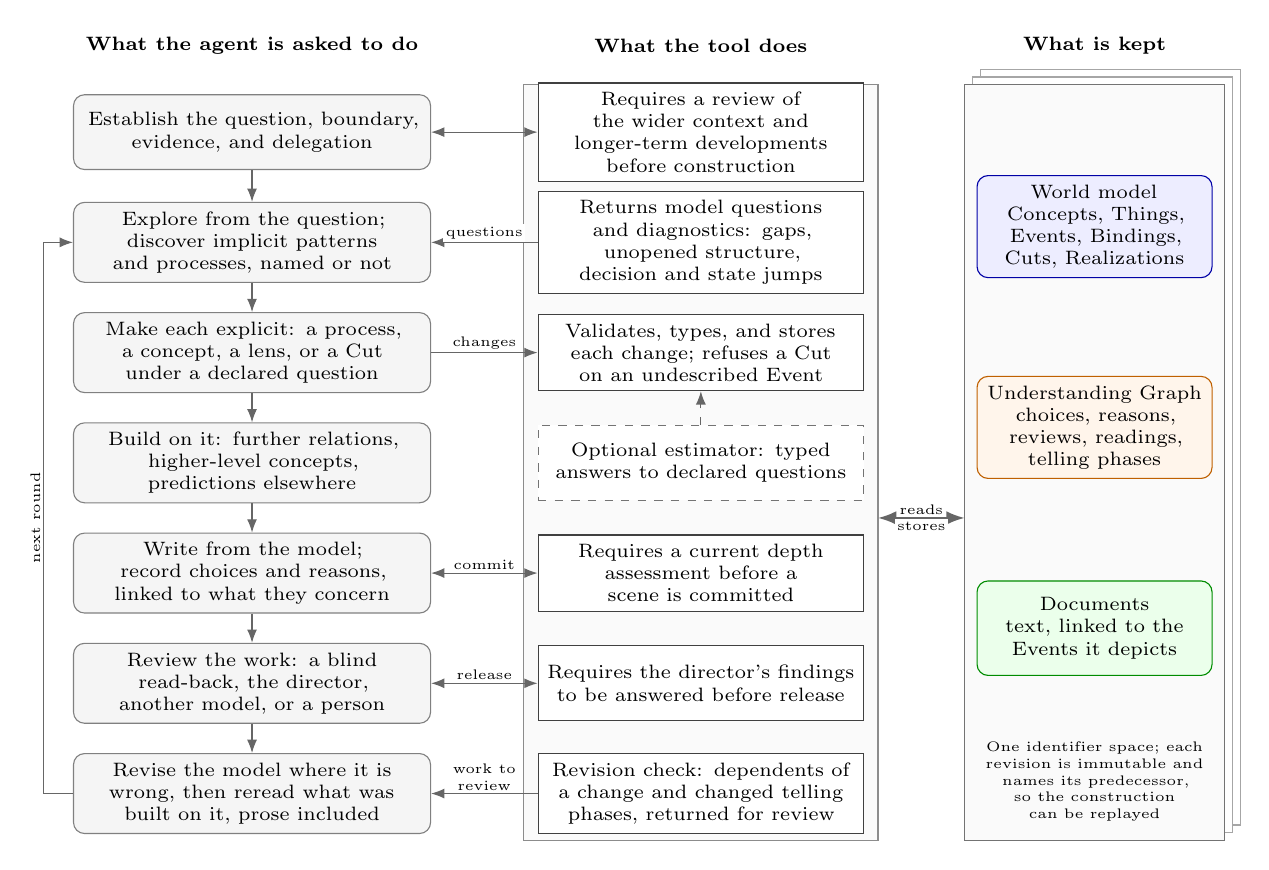
\begin{tikzpicture}[
  x=1cm,y=1cm,>=Latex,
  head/.style={font=\scriptsize\bfseries,align=center},
  ask/.style={draw=black!50,rounded corners,fill=black!4,align=center,
    font=\scriptsize,text width=4.3cm,minimum height=.95cm},
  tool/.style={draw=black!75,fill=white,align=center,
    font=\scriptsize,text width=3.9cm,minimum height=.95cm},
  optional/.style={tool,dashed,draw=black!55},
  surface/.style={rounded corners,align=center,font=\scriptsize,
    text width=2.75cm,minimum height=1.2cm},
  world/.style={surface,draw=blue!65!black,fill=blue!7},
  author/.style={surface,draw=orange!75!black,fill=orange!8},
  render/.style={surface,draw=green!55!black,fill=green!8},
  flow/.style={->,thin,draw=black!60},
  label/.style={font=\tiny,fill=white,inner sep=1pt,align=center}
]
\hyphenpenalty=10000 \exhyphenpenalty=10000
\node[head] at (2.35,1.1) {What the agent is asked to do};
\node[head] at (8.05,1.1) {What the tool does};
\node[head] at (13.05,1.1) {What is kept};

\node[ask] (s1) at (2.35,0) {Establish the question, boundary,\\evidence, and delegation};
\node[ask] (s2) at (2.35,-1.4) {Explore from the question; discover
  implicit patterns and processes, named or not};
\node[ask] (s3) at (2.35,-2.8) {Make each explicit: a process, a concept,
  a lens, or a Cut under a declared question};
\node[ask] (s4) at (2.35,-4.2) {Build on it: further relations,
  higher-level concepts, predictions elsewhere};
\node[ask] (s5) at (2.35,-5.6) {Write from the model; record choices and
  reasons, linked to what they concern};
\node[ask] (s6) at (2.35,-7.0) {Review the work: a blind read-back, the
  director, another model, or a person};
\node[ask] (s7) at (2.35,-8.4) {Revise the model where it is wrong, then
  reread what was built on it, prose included};
\foreach \a/\b in {s1/s2,s2/s3,s3/s4,s4/s5,s5/s6,s6/s7}
  \draw[flow] (\a) -- (\b);
\draw[flow] (s7.west) -- (-.3,-8.4) --
  node[label,rotate=90,above]{next round} (-.3,-1.4) -- (s2.west);

\draw[draw=black!45,fill=black!2] (5.8,.6) rectangle (10.3,-9.0);
\node[tool] (t0) at (8.05,0) {Requires a review of the wider context and
  longer-term developments before construction};
\node[tool] (t1) at (8.05,-1.4) {Returns model questions and diagnostics:
  gaps, unopened structure, decision and state jumps};
\node[tool] (t2) at (8.05,-2.8) {Validates, types, and stores each change;
  refuses a Cut on an undescribed Event};
\node[optional] (t3) at (8.05,-4.2) {Optional estimator: typed answers to
  declared questions};
\node[tool] (t4) at (8.05,-5.6) {Requires a current depth assessment
  before a scene is committed};
\node[tool] (t6) at (8.05,-7.0) {Requires the director's findings to be
  answered before release};
\node[tool] (t5) at (8.05,-8.4) {Revision check: dependents of a change and
  changed telling phases, returned for review};
\draw[flow,dashed] (t3) -- (t2);

\draw[flow,<->] (s1.east) -- (t0.west);
\draw[flow] (t1.west) -- node[label,above]{questions} (s2.east);
\draw[flow] (s3.east) -- node[label,above]{changes} (t2.west);
\draw[flow,<->] (s5.east) -- node[label,above]{commit} (t4.west);
\draw[flow,<->] (s6.east) -- node[label,above]{release} (t6.west);
\draw[flow] (t5.west) -- node[label,above]{work to\\review} (s7.east);

\foreach \d in {.2,.1}
  \draw[draw=black!35,fill=white] (11.4+\d,.6+\d) rectangle (14.7+\d,-9.0+\d);
\draw[draw=black!55,fill=black!2] (11.4,.6) rectangle (14.7,-9.0);
\node[world] (r1) at (13.05,-1.2) {World model\\Concepts, Things, Events,
  Bindings, Cuts, Realizations};
\node[author] (r2) at (13.05,-3.75) {Understanding Graph\\choices, reasons,
  reviews, readings, telling phases};
\node[render] (r3) at (13.05,-6.3) {Documents\\text, linked to the Events
  it depicts};
\node[font=\tiny,align=center,text width=2.9cm] at (13.05,-8.25)
  {One identifier space; each revision is immutable and names its
  predecessor, so the construction can be replayed};
\draw[flow,<->,thick] (10.3,-4.9) -- node[label,above]{reads}
  node[label,below]{stores} (11.4,-4.9);
\end{tikzpicture}
\caption{The construction loop. Left: what the shared instructions ask the
calling language model to do. The order is a guide rather than a fixed
sequence; any step may lead back to exploration, and each round builds on the
account the previous one left. Middle: what deterministic tool code does. It
validates and stores every change, returns questions after each one, refuses
gated operations until the required reviews exist and their findings are
answered, and lists the work a revision makes due. The estimator is optional,
and the scene and release gates belong to the storytelling add-on. Right: the
one versioned record that every step reads and changes through the tool. The
tool checks records and their declared links; it does not supply the
interpretations or certify that an account is adequate.}
\label{fig:construction-loop}
\end{figure}


\subsection{MCP entry points and operations}

The interface supplies resources, prompts, and tools. Resources carry the papers,
operational guides, and examples; prompts assemble a starting task for the
calling language model; tools inspect records, prepare proposals or review
packets, and apply explicit changes. The general tools, including memory, are
always available;
storytelling and mechanism search are optional workflows that may be enabled
together. Workflow is distinct from modeling purpose: observation, forecasting,
counterfactual analysis, source reconstruction, person reflection, or creative
fiction sets the evidence and authority contract. The language model supplies
substantive interpretations; a prepared task is not an executed review, and a
review packet is not an accepted result. Agents begin with operational guidance and purpose-specific instructions;
the papers remain optional references. The guidance states the construction and
preservation contracts, while model validation and recorded resource access
do not prove comprehension. Tool names, parameters, and startup and continuation
procedures are documented in the
\href{https://github.com/emergent-wisdom/meaning-model/blob/main/mcp-server/README.md}{MCP server guide}.

Registering a model revision is distinct from advancing a runtime world. A roll
executes the declared laws to propose one complete continuation; inspection and
comparison do not accept it, and acceptance commits one candidate against its
expected parent. Adopting a registered revision into a running world is an
authored change under compatibility checks. Neither makes an authored
description an executable law or establishes its truth.

\subsection{The language model, estimator, and storage loop}

The division of work separates open-ended construction from bounded evaluation.
The language model develops process descriptions and candidate explanations,
writes Document Nodes, and records concise assessments and
revision reasons in Understanding Nodes. It also designs the numerical
questions and revises inadequate categories. An optional estimator supplies
structured judgments for those questions. Deterministic tool code validates,
types, and stores the results with their coordinates and provenance, avoiding a
second language-model pass that manually transcribes each value and graph edge.

The current optional provider is TypeSafe's
\href{https://docs.typesafe.ai/introduction}{Jev}, which answers declared
questions with typed options at call time. Answering a bounded question with a
classifier's decision rather than generated text predates Jev: SetFit, for
example, fine-tunes a compact sentence encoder and fits a classification head
for a fixed label set, without prompts~\cite{tunstall2022setfit}. The estimator
is a replaceable instrument. It does not supply the open-ended process
descriptions, a universal ontology, or an independently verified account of
reality, and its use is independent of enabling storytelling.

The general workflow is:
\begin{enumerate}
  \item Establish the question, system boundary, time basis, evidence, and
  delegation already agreed with the user. Review the enclosing system and
  longer-term developments before selecting sector-level and focal processes;
  examine feedback from those processes into the broader account. Select a
  minimally adequate account rather than attempting exhaustive construction.
  \item Supply a compact scaffold of referents, processes, events, sources, and
  descriptions. The tool expands the initial model and graph. Supplied numerical
  measurements retain their units; missing states remain unresolved unless an
  explicit estimation question is answered.
  \item Obtain typed process-value proposals for the selected process coordinates.
  Validate their types, bounds, question identities, evidence cutoffs, and access
  scopes. Preserve the exact questions, answers, and model revision for review.
  \item Review and apply the exact construction proposal, or record a later
  estimate and its attributed review in the graph. Understanding Nodes explain
  what was retained, questioned, or revised. A retry must not silently regenerate
  a different set of values.
  \item Use the account, inspect missing evidence and competing explanations,
  and deepen or revise the processes where this improves the inquiry. Preserve
  earlier versions and reassess affected interpretations and documents. The
  accepted account becomes context for the next round: its explicit processes,
  relationships, and concepts support further inference and abstraction, as well
  as constrain proposed detail.
\end{enumerate}

Before external estimation or construction, the compact builder requires an
attributed review of the wider context and the longer-term developments behind
the focal question. Each is represented, left explicitly unknown, or excluded
with a reason, and the review is stored as Understanding Nodes. Recording the
review does not establish that the account is explanatorily adequate. The
builder also requires consideration of whether authored numerical judgments, a
finer conceptual decomposition, or a change of meaning across dates or
perspectives would help; that consideration does not require invented scores,
finer categories, or a claim that meaning changed. A long event is not a sampled
numerical trend: numerical histories require values at explicit coordinates
with their evidence cutoffs.

The compact construction tool and typed estimation exchange are distinct
operations. Initial estimates can be explicitly adopted as estimated initial
claims. Subsequent provider estimates and reviews can be recorded durably in
the graph without advancing accepted runtime history. A review approval does
not turn an inferred state into an observation; runtime observations retain the
ordinary candidate and acceptance path. Multi-operation construction reports
partial completion rather than claiming transactionality across separate model,
graph, and world writes.

A probability distribution over answer categories is not automatically an
attention allocation, a physical share, or a causal law. Rubric-derived scalar
values require declared numeric anchors and units; their source distribution
and uncertainty remain inspectable. Public statements support attributed
accounts of a person's expressed views, not privileged access to private
reasoning. Source selection and question design remain substantive modeling
choices even when numerical evaluation is automated.

\subsection{Lenses and revision review}

The core lens tools make a revisable question reusable across records. A lens
records the question and its current alternatives, with readings located under
the appropriate holder's root and linked to what is read. Quantitative answers
belong to those reading Events as Cuts, retaining the question, unit, and
remainder. They do not acquire the authority of the world record they interpret.
Diagnostics expose unanswered readings and possible finer openings. A useful
answer can be opened through conditional Cuts, or the agent can record why the
present resolution suffices or the lens does not apply. Templates are optional.
Changed source text or lens versions can make readings stale; the workflow
supports reassessment through a configured estimator. The procedure records
interpretations, not a universal taxonomy.
Source-text freshness distinguishes an unchanged recorded signature from
changed text requiring review, an unresolved source, and an untracked basis.
An unchanged signature is neither a new assessment nor a
certificate that the reading is true.

After a model revision, a check compares specified model versions. It follows
declared dependencies to conditioned Cuts, draws made from changed weights,
readings of rewritten text, and passages that render a changed record. It also
lists for review Events connected through recognized causal relations and
visible understanding notes directly linked to changed records; an
\texttt{about} link does not make a note a dependent. Telling phases are
checked separately, against the current text and reading order, independently
of which model revisions are compared. The check returns work to review,
without repairing or certifying the construction. Coverage is limited to
recognized changes and visible links. In the current prototype, changes to
concept definitions require manual review of their linked dependents.
Semantic agreement, disclosure, and dependency completeness still require
assessment.

\subsection{Storytelling over the same core}

The storytelling add-on adds author and character models, overall life trends,
numerical trajectory exploration, scene preparation, and prose review. Intake
separates which initial parameters the user supplies from how involved they
wish to remain during writing. A fully delegated language-model author may
perform the construction and writing loop within that brief. It writes the
prose and evaluates author and character voice against
specific text and modeled processes, recording those assessments in
Understanding Nodes.

A human author can instead write the work and use the language model for
feedback. The model explores the text and its underlying processes, linking
observations and proposals to evidence in the work and, where available, its
modeled world. Authorship and creative decisions remain with the human;
feedback does not accept a model revision or rewrite the prose. The same
open-ended inquiry applies without imposing a fictional author persona or a
fixed literary form.

The model is intended to do more than check prose. It supplies material:
modeled dates, alternatives, and quantities become the content of scenes, and
because a decision needs represented alternatives and causes, the constructor
must supply specific constraints rather than atmosphere. It serves as the
writer's memory across a long work: dates, sums, and who knew what at each
point are read from the model and the disclosure records at every edit. It
keeps revision local: declared dependencies name the facts, phases, notes, and
passages that a change affects. Its diagnostics can also point to where the
story turns, since a ranking of decision and state jumps is derived from the
model before any reader responds. The guidance also asks the writer to compress
the story into a sentence, a paragraph, and a page, and to write down the ideas
the work means to convey with a strategy for conveying each, which a blind
read-back can test. The sentence
is the coarsest
description of the work and a first test of whether it is interesting; as the
telling grows, it should still fit that sentence, or the sentence is revised
explicitly, as with any protected coarse answer. These are design expectations;
the prospective comparison tests them.

Before preparing a scene for commitment, the add-on requires a current
model-depth assessment of the stored plan and its explanatory evidence.
The server checks the referenced records and source identity; the calling
model judges sufficiency. After substantial drafting or revision, a separate
actual-prose review considers purpose, realized author voice, and each relevant
character's speech and actions against the modeled life and situation.
Its literary advice is advisory, not a quality gate. Exploratory drafts and
questions may precede either review; neither imposes a fixed character taxonomy
or requires an explanation for every ambiguity.

A director review assesses the world before the first scene, and the draft
before release, against stated principles: for instance, that no death or
accident does the plot's work, that the route passes through the model's
largest jumps, and that each recorded idea reaches the reader. The reviewer
judges each principle against the work's form, purpose, and context, and may
explain why it does not apply. Each failing finding names the model or prose
change it needs. Several of its principles
were distilled from understanding notes recorded while the Book was
constructed. Release requires a director
review of the current prose and a later answer to every failure found at either
stage, with a changed model or a fresh passing review of changed prose where the
finding requires it. The server checks these records; whether a repair
succeeded remains a judgment.

Scenes can contain ordered, independently editable passages. Shared graph
editing supports splitting, merging, moving, reordering, and local text
revision while retaining predecessor versions. A separate deepening pass can
revise an existing work and its supporting model. These mechanisms organize
construction and review; they do not establish distinctive voice, literary
quality, or semantic alignment merely by accepting a structurally valid record.
General-purpose modeling does not require author personas, dramatic goals, or
any other literary vocabulary.

New or changed prose declares which Events it depicts, or records why it
depicts none. Revision and release checks follow these declarations; they do
not infer depiction from similar words or establish that the prose is faithful.
The story release operation widens access to selected prose without changing
the access scopes of other authoring records.

Depicting an Event does not disclose all its facts or motives. Disclosure plans
distinguish what a reader can already know, what a passage reveals, and what
remains withheld or ambiguous, separately from character knowledge in world
time. They use existing passage identities, reading order, linked author
records, and optional document spans. These attachments support revision as
text grows or is split; their meaning and scope still require review after an
edit. This introduces no new clock system or required numerical reader model.

Optional telling-process records describe qualitative phases of disclosure,
attention, tension, or another question chosen for the work. These are attributed
assessments recorded as UnderstandingNodes, interpreting the realized text
separately from a disclosure plan's intended revelation and withholding. Each phase names a
stable document span and quotes its supporting passages; the record retains
its holder, reviewed text hashes, and reading order. The viewer projects these
phases in document position, with current, needs-review, or unresolved status
when the text, order, or accessible span changes. These are attributed readings
of how a work unfolds, not measured reader psychology or simulated world time.

\subsection{The construction record}

The workflows treat the model and its Understanding Graph as the modeler's
understanding rather than a report about it. Work that is done and not recorded
cannot be continued by another agent, and a thought that is not linked to what it
concerns cannot be found again. Every Event that parents a Cut therefore carries a
description of what happens in it, because the Cut's question and weights are read
against that Event; the tools refuse or block Cuts on undescribed Events. Choices,
ideas, predictions, voice decisions, and their reasons become UnderstandingNodes held
by a named holder and linked to the exact records they concern, down to a single Cut
answer. Reviews by other models, blind readers, estimators, or people are
UnderstandingNodes held by the reviewer, with the revision and text it read. Because
every stored revision is immutable and names its predecessor, the recorded
construction can be replayed: the model revisions each step adopted and any
reasons, notes, and reviews saved with them, with each note beside the records
as they were when it was written. Replay cannot recover unrecorded reasoning
or revisions excluded from an export. An agent continuing an unfamiliar story or
model recovers its history through replay and an outline before changing it.
When the exact previously read revision and its context are retained, the agent
reads subsequent changes and the records relevant to the current work. An outline
presents the current state at a chosen depth. The
construction also travels: a full-history export holds the recorded model
revisions and each graph revision as its change, and another engine rebuilds it with the same hashes,
so the replay there is the same replay.

A bundled read-only viewer presents the same records: coarse and detailed views
retain the addressed wholes; spatial views use declared positions in explicit
frames, while other layouts claim no physical geography; connections to Events,
passages, and understanding follow recorded links; author and reader lives keep
their own worlds and times; and reading order remains distinct from world time.

\subsection{Mechanism search through invented worlds}

The optional alien add-on implements the world-diversity search of Ontology of
the Alien over the same graph~\cite{westerbergOntology2026}. A target-blind
builder turns a seed word into an invented world; a purpose-blind solver addresses
the problem inside that world; a compiler states the operative causal relation in
the problem's own domain. The server writes each role's task, stores its exact
text, and records every output against the task it answers. Curators maintain
three revisable ontologies: mechanism families, claimed outcomes, and causal world
regimes. Their partitions are specializations under a named lens, not expressive
decompositions. A new family is admitted only when the recorded equivalence test
says the primary causal operator changed; the judgment itself remains the
curator's. Diagnosis of the ontologies, including family and outcome
combinations that no candidate yet realizes, informs the commission of the next
world. A transfer maps a mechanism's roles onto records of the target model and
states where the analogy breaks; a graded fit is a fit Cut with its own remainder.

An alternative explorer works directly from the target problem, with or without
a random-word cue. Both routes can use no population context, an inventory of
earlier approaches to avoid, or the curated map. The add-on records these
conditions so their results can be compared under matched budgets; merely
supporting the alternatives does not establish which works better. The cited
Ontology of the Alien study did not run the uncued direct explorer without
population context; running that condition would extend the study rather than
replicate a reported condition.

These records organize ideation. A world is a textual thought experiment, not a
simulation, and a transfer records an idea and its mapping, not evidence that the
idea works. The add-on implements the world-population ontology and graph-directed
world commissioning that Ontology of the Alien proposes. A second judge from another
model family can answer each curator decision's comparison without seeing its
reasons, which addresses that paper's single-coder limitation, and target-blind
worlds can be exported as a library and imported into later searches. Whether governed world
coverage yields more useful mechanisms than unguided generation remains that
paper's open experiment.

The architecture is intended to reduce repetitive language-model work through
batched judgments and automatic ingestion. An end-to-end efficiency claim must
include evidence preparation, question design, provider calls, validation,
review, and repair, compared on equivalent tasks. Structural tests or a single
live provider run do not establish lower total cost, faster completion,
calibrated judgments, predictive accuracy, or superior fiction.

\section{What Changes When Works Are Constructed}
\label{sec:implications}

If books, films, and game worlds come to be constructed this way, a work is no
longer its text alone. A book becomes one route through a modeled world, whose
reading order passes through Events that exist whether or not a scene shows
them; the storytelling guidance already treats a story as a small window onto a
world modeled far beyond it. A film, a game, a sequel, a translation, or an
adaptation becomes another route through the same world, and continuity between
them becomes partly checkable, where depiction and dependencies are declared,
rather than something curated by memory. Readers and players could open the world behind a work: read a
secondary person's life from its beginning, follow a process the story only
glimpsed, or ask what a character knew on a given day, with each answer
attributed to whoever holds it.

Game worlds change most directly. A world could stay coarse but consequential
everywhere and open detail where a player goes, as the harvest example in the
Introduction describes. Its people would have modeled lives whose decisions
consult their trajectories, and shared facts would stay the same for every
player. Procedural generation and level-of-detail simulation already produce and run
large worlds~\cite{brom2007,sunshine2010}; what could change is coherence at that
scale, because progressive resolution and a shared construction medium let detail
be constructed when it matters and checked against what is already committed.

Authorship can shift toward direction. The human who commissions a work chooses
what it should convey, the strategy for conveying it, and what makes it worth
reading, and judges the result; the language model can construct the world and its
telling under those commitments. Because the construction record keeps choices,
reasons, and reviews with the records they concern, who decided what becomes
inspectable where it is recorded, and a revision can be traced to the commitment that caused it.
Criticism could gain further evidence: the ideas the work was built to convey,
the strategy recorded for each, and blind read-backs that test which of them a
reader recovers.

The worlds also become learning material. Construction histories pair a
situation with the refinement, repair, or stopping decision taken, the kind of
example from which a system might learn to think in explicit, consistent worlds,
as Life Simulation proposes (Section~\ref{sec:companion}). Modeling fictional people from where their lives
begin may also be practice for the harder, evidence-bound task of understanding real
people.

The changes carry risks. One grammar and one model's implicit priors could
narrow the range of worlds, the Median Trap that the world-diversity search of Ontology of the Alien is
designed to counter~\cite{westerbergOntology2026}. Comparative numbers can
lend false precision to a poor question, and a highly coherent invented world can
persuade more than it should. Real people need protection: the storytelling
guidance asks that living people and real organizations not take part as
characters, and the director review checks it. Some art
depends on what is left unsaid. The model can record a motive fully while the
telling withholds it, which is a disclosure choice rather than an unresolved Cut;
where the author leaves something genuinely open, that openness can be recorded as
such. None of these
consequences is demonstrated here beyond \emph{The Book of Conditions}; they describe
what the method is for.

\section{Related Work}
\label{sec:related}

Prototype and family-resemblance accounts reject the assumption that every
category is defined by one set of necessary and sufficient surface features
\cite{roschMervis1975}. The Meaning Model likewise permits graded fit Cuts,
exemplars, boundary cases, and plural models. Only its deepest grounding option
uses an inspectable process-based concept model.

Structure-mapping theory treats comparison as an alignment between relational
systems \cite{gentner1983structureMapping}. Realization borrows that discipline:
role alignment is recorded before component fit is aggregated. The present
proposal is narrower computationally; it does not claim a complete cognitive
theory of analogy.

Normalized attention has precedents: Nosofsky's exemplar model allocates
nonnegative weights summing to one across perceptual dimensions for
categorization \cite{nosofsky1986attention}. The proposed methodological use here
is recursively refinable, question-relative conceptual allocations in evolving
worlds, coordinated with construction and revision.

Dempster--Shafer theory permits basic probability mass to remain assigned to
sets of possibilities, including the whole frame, without distributing it
among individual possibilities \cite{shafer1976evidence}. The Meaning Model's
remainder instead retains the unresolved share of a question-local unit, such
as attention or duration; it is not generally evidential mass, and the grammar
does not adopt Dempster's rule for combining evidence.

Frame semantics and script accounts organize meaning around structured roles
and characteristic situations or event sequences
\cite{fillmore1976frame,schankAbelson1977scripts}. Process-based concept models can
make those roles and sequences refinable through the same thing-event grammar
used for a token world. Conceptual spaces instead emphasize geometric regions
and similarity \cite{gardenfors2000conceptualSpaces}; such a space can be
attached as an external domain model, while Realization links and fit Cuts
preserve the grounding, alignment, perspective path, and local alternatives
used.

Process ontology and event mereology motivate taking temporal entities and
their parts seriously \cite{whitehead1978process,savellos2000events}.
The continuant--occurrent and SNAP--SPAN tradition likewise distinguishes
entities that remain identifiable through change from processes extended in
time, and explicitly relates a continuant to the occurrent that is its life
\cite{grenonSmith2004snapspan}. The Meaning Model's Thing--lifecycle pairing is
in that lineage, while its local cuts and plural concept grounding address a
different construction problem.
Object-Process Analysis places objects and processes in one recursively scalable
systems account \cite{dori1995opa}. Descriptions and Situations distinguishes a
reusable description from a situation satisfying it
\cite{gangemiMika2003dns}. The Meaning Model's distinctive choice is the local
one-unit cut with explicit remainder, ancestry-derived perspective, plural concept
grounding, and conservation under progressive refinement.

Narrative systems already maintain worlds. Inform tracks rooms, objects,
containers, and interaction scope \cite{nelson2001inform}; bAbI tests synthetic
location and relation updates \cite{weston2015babi}; ProPara annotates entity
existence and location changes \cite{dalvi2018propara}. EvolvingWorld couples
persistent character and global state in literary role-play
\cite{zong2026evolvingworld}. Narrative World Model extracts typed temporal memory
from accepted prose and invalidates downstream records after edits; its reported
evaluation concerns narrative question-answering, with generation evaluation
left for future work \cite{saifullah2026narrativeworld}.

Hierarchical and model-assisted authorship also have direct precedents. DOC
expands hierarchical outlines and controls passages against them
\cite{yang2023doc}. DOME interleaves detailed planning and writing with temporal
knowledge-graph memory \cite{wang2024dome}. Generative Agents combines recorded
experiences, reflections, and plans to produce behavior \cite{park2023agents}.
The Meaning Model therefore does not claim to introduce planning, graph-backed
storytelling, or reflective characters. Among the systems compared in
Table~\ref{tab:predecessor-contracts}, its distinction is recursive
inference anchored in explicit world structure under a shared preservation
contract: a coarse world remains consequential before
its details exist; an opening must satisfy declared fine-to-coarse checks or
trigger explicit revision. Local comparative person Cuts and versioned concept
groundings participate in that same construction rather than forming unrelated
annotations.

Making implicit knowledge explicit also has a long history. Knowledge
engineering elicited experts' knowledge into the rules of expert
systems~\cite{feigenbaum1977art}, and Cyc hand-encoded commonsense concepts and
axioms from 1984 on~\cite{lenat1995cyc}. Both depended on people to articulate
what they knew, and tacit knowledge resists that~\cite{polanyi1966tacit}. Here the
language model is asked to articulate its own understanding, recursively and at
the scale of a long work, under a grammar that quantifies meaning comparatively and
preserves commitments across openings, and the result is a world and its telling built for one inquiry or work. The
Meaning Model's two linked architectural contributions, progressive resolution
and a shared construction medium, together connect discovered concepts,
quantitative commitments, recursive refinement, and coordinated revision in one
inspectable account. The comparison below locates each part among its
precedents; to our knowledge, no earlier system specifies this complete operation
for a language model constructing and revising its own explicit world model.

The cross-scale pattern has important precedents. Holling's panarchy account
links faster, smaller adaptive cycles with slower, larger ones: local
disturbances may propagate upward, while accumulated structures and resources
shape reorganization below. He also describes departures from the cycle
\cite{holling2001complexity}. This is a close conceptual relative, not evidence
that every represented process must complete the same stages.

Dalio's historical practitioner account connects expectation, surprise, and
revision across debt, conflict, natural disturbances, and human adaptation
\cite{bridgewaterDalioGrantham2022}; neither its causal interpretation nor a
fixed historical cycle becomes a law of the grammar.
The useful intuition is that earlier historical cases can help revise present
expectations after an unexpected outcome.

At everyday timescales, event-segmentation theory connects perceived boundaries
with prediction error and considers simultaneous finer and coarser event
models \cite{zacksEtAl2007event}. These accounts supply related hypotheses at
different scales, not a single established mechanism from perception to
history. The Meaning Model makes their processes, expectations, responses,
and cross-scale explanations addressable for comparison. Change-point, jump--diffusion,
mean-reverting, self-exciting, and hybrid models are downstream candidates for
Life Simulation rather than alternative record grammars
\cite{killick2012changepoints,merton1976jump,uhlenbeckOrnstein1930,
hawkes1971,goebel2009hybrid}.

Semantic Spacetime treats promises, agents, names, and scale as foundational to
functional knowledge representation \cite{burgess2016semanticSpacetimeIII,
burgess2017cognitiveReasoning,burgess2020narrativeII}. The present grammar
combines multi-scale semantic graphs with explicit model commits and
question-local composition.

The contribution is architectural and methodological: coordinated refinement
and revision of world commitments, concept interpretations, authoring reasons,
and prose, with each explicit account supporting further inference and
abstraction. A revised success criterion, for example, can require rechecking a
trial's assessment, the rationale for expansion, and the passages expressing
both. The relevant comparison unit is that complete operation: what may remain
unconstructed, which commitments an opening protects, and how a revision affects
the connected account. An antecedent for graphs, normalized allocations, or
revision alone does not settle whether this method has already been specified;
neither does their combination establish priority by itself.
Table~\ref{tab:predecessor-contracts} therefore compares the contracts of that
operation across the closest systems, as their own papers describe them. Each
supplies part of it: outlines and plans commit coarse structure before detail,
a controller steers passages toward outline items, a verifier checks candidate
chapters against stored state, republishing invalidates dependent memory,
reflection builds higher-level thoughts on stored records, and an open schema
infers categories for each work. Generative Agents comes nearest to the
discovery loop: its reflection prompt asks for high-level insights together with
the memories that support them \cite{park2023agents}. Those insights remain
text memories. The Meaning Model asks the constructor to make discovered
concepts and processes trackable in the grammar that holds their instances, so
that they can be followed over time, tested elsewhere, and revised under the
preservation contract. Narrative World Model comes closest to the whole
operation, but it records memory only from finalized prose, in a specified set
of narrative fields. None of those compared specifies the complete operation.

\begin{table}[htbp]
\centering
\scriptsize
\begin{tabularx}{\textwidth}{@{}>{\raggedright\arraybackslash}p{0.12\textwidth}YYYYYY@{}}
\toprule
System & Coarse commitments before detail & Detail checked against them & A revision rechecks its dependents & Explicit records support further inference & Accounts kept per holder & Categories constructed and revised \\
\midrule
DOC \cite{yang2023doc} & Outline expanded before drafting (\S3.2) & Controller steers passages toward outline items (\S3.3) & Not described & Inferred character facts reused in later passages (\S3.2) & Not described & Not described \\
DOME \cite{wang2024dome} & Rough outline, then detailed outlines (\S4.1) & Retrieval reduces conflicts; conflicts measured after generation (\S4.2--4.3) & Later outlines adjusted forward (\S4.1) & Extracted quadruples retrieved for planning (\S4.2) & Not described & Not described \\
Generative Agents \cite{park2023agents} & Day plan decomposed into finer actions (\S4.3) & Reactions regenerate the remaining plan (\S4.3) & Not described for memories or reflections & Reflection trees over observations and reflections (\S4.2) & Each agent's own memory stream (\S4.1) & Not described \\
Narrative World Model \cite{saifullah2026narrativeworld} & No: memory records finalized prose (\S3.1) & Candidate chapters checked for unsupported state changes (\S3.4) & Republishing invalidates dependent memory (\S3.1) & Recursive question answering over stored state (\S3.4) & Character knowledge and unknowns (\S3.2) & Specified narrative fields; revision not described (\S3.2) \\
EvolvingWorld \cite{zong2026evolvingworld} & Not described & Not described & World state updated after each interaction (\S3.2) & Stored states inform scene selection and actions (\S3.2) & No: one shared objective state (Limitations) & Dimensions inferred for each book (\S1) \\
Inform \cite{nelson2001inform} & No: world declared in the source & Actions checked against world rules (\S24) & Not described & Not described & Scope limits what the player addresses (\S24) & Not described \\
Meaning Model & Protected coarse answers & Close, or explicit revision & Declared dependents across world, concepts, reasons, and prose & Records and concept models anchor further opening & Perspective by containment & Versioned groundings with supersession \\
\bottomrule
\end{tabularx}
\caption{Contracts of the complete revision operation in the closest systems,
as described in their own papers. ``Not described'' means the source does not
describe the contract, not that the system could not support it. The Meaning
Model row states specified contracts;
Table~\ref{tab:book-enforcement-boundary} gives what the prototype
implements.}
\label{tab:predecessor-contracts}
\end{table}

The Book partially demonstrates feasibility, while
comparative literary benefit, learning gains, and computational savings remain
untested.

\section{Limitations and Research Boundary}
\label{sec:limitations}

Normalization enforces accounting consistency, not truth. A cut can ask the
wrong question, choose misleading children, or encode an LLM's bias with false
precision. A concept hierarchy, exemplar set, or concept model can privilege
one culture or perspective. Role alignment can manufacture apparent similarity.
The recorded ancestry, remainder, evidence, provenance, and grounding version
make these judgments inspectable rather than eliminating their biases.

The Book's concept vocabulary and exemplar anchors are not yet validated.
Definitions can drift, rankings of alternatives under one Cut question can be
inconsistent, and sparse exemplars can hide boundary cases. Concept induction
can overfit examples or proliferate names until comparison becomes meaningless.

The mixture law applies only where compatible Cut questions warrant it.
Occurrence, logical constraint, topology, and causal intervention remain Event
or domain relations. Cut shares express a declared comparison, not freestanding
intensity. Quantities with independently interpretable units or declared
measurement protocols remain world data,
whether measured, inferred, or fictionally authored. The grammar does not replace
physics, economics, biology, geometry, or any field with units and specialized laws.

Book-specific person, emotion, motivation, and strategy vocabularies have not
been validated as complete, culturally portable, or optimally independent.
They are expected to change through the iterative construction and testing
practice described above. Event and period boundaries are likewise
model commitments rather than naturally labeled facts. The grammar makes these
choices inspectable; it does not turn them into a psychology or a dynamical law.

Root and surface separation preserve attributions but do not reveal hidden minds.
Historical character interiors remain authored interpretations. Human
explanations inherit hindsight, narrative compression, and over-attribution to
character. A model trained on them may become better at predicting people or
merely better at producing plausible stories about them.

Finally, recursive refinement is not empirical utility. A strong language model
may already maintain equivalent structure implicitly. The Book comparison must
establish whether explicit records improve coherence and read-back enough to
justify their construction and maintenance cost.

\section{Relation to Life Simulation and the Wider Program}
\label{sec:companion}

Life Simulation uses completed or ongoing worlds to study the generation,
inference, and learning of process histories. Continuations may come from an
LLM, an authored account, a simulator, or a fitted function; no compact
dynamical law is required. Comparing continuous, discrete, or hybrid laws is
one research task within that broader method. Its process-aware models are
intended for games, scientific or social simulation, exploring unfamiliar
causal mechanisms through Ontology of the Alien, organizing problem-solving
capabilities through Fractal Intelligence, and alignment-facing curricula
\cite{westerbergLifeSimulation2026}.

This is not a one-way handoff. Life Simulation can propose a continuation or a
predictor; Meaning Model construction rules still govern its representation,
acceptance, and effects on dependent records and text. Meaning Model read-back
checks what a passage says about its source world. Life Simulation's inverse
task asks what hidden processes observations support, and whether inferred
accounts predict later evidence or transfer beyond their construction setting.
Together the two proposals support a feedback loop: construct a world, render
observations, infer an account from the available evidence, compare its
predictions with later evidence, and revise the account before constructing
further. Correction may change an Event, a decomposition, or a Concept's
grounding, rather than merely add detail. The Meaning Model makes those changes
addressable and preserves their history; Life Simulation specifies learning
objectives and independent tests. Agreement with a construction's own rendering
alone does not validate its account of reality.

The inner-life ambition connects three levels of this loop. \emph{In the
story}, a character holds a model of the world and estimates of other
characters, and acts from that perspective. \emph{In construction}, the
modeler builds and revises those character models, recording its own estimates
and reasons separately. \emph{In the long run}, a trained system could use the
same distinctions to estimate real people's changing perspectives from
available evidence. The first two levels supply candidate learning material
for the third. At each level, an estimate retains whose account it is, what it
concerns, and what evidence was available when it was made. In a constructed
world, it can be scored against the stipulated character state when that target
becomes available. For real people, later reports, actions, and observations
provide fallible evidence against which predictions and uncertainty can be
assessed; they do not reveal a complete private state. Preserving the original
estimate and its cutoff makes inner-state estimation improvable, instead of
replacing an earlier guess with a more convincing retrospective account.

A connected Meaning Model of actual world history and geography can deepen as
evidence arrives. Sources share supported identities while retaining separate
claims, evidence, and disagreements. Regions and centuries can open into
institutions and lives without equal detail everywhere, and new evidence can
revise earlier accounts, not merely add detail, with event and revision times
kept distinct. Acceptance does not establish historical truth; fictional worlds
retain separate contexts. Meaning Model supplies the representation and
revision contract; Life Simulation develops corpus-wide construction,
interpretation, and training. At corpus scale, the tool would need incremental
ingestion, selective retrieval, and dependency-aware revision over one logically
connected address space, potentially distributed across storage systems. New
material would link to supported identities and source records; refinement
would open only the processes needed for an inquiry. Versioned dependencies
would identify derived views affected by a correction for explicit revision or
stale marking, while preserving their source records and prior versions. Access rules, perspective boundaries, temporal
cutoffs, and the selected profile's commitment and recomposition contracts must
hold across storage boundaries. These are proposed extensions of the tool, not
additional grammar forms or an implemented corpus-scale system.

Imagining the Corpus pairs source text with visual sequences and persistent
state updates for joint prediction \cite{westerbergImagining2026}. Entangled
Alignment supplies the recommended Reader-based training approach: a Teacher
generates questions, interpretations, and revisions from the source prefix and
the Reader's prior Understanding Graph, and a Student would be trained to
predict selected source continuations, Reader updates, or graph operations
\cite{westerbergEntangled2026}. In its full proposed alignment treatment, each Reader
thinking block starts with the same complete Reader Core, seven first-person
commitments including care and wisdom, and their application to the situation is
called Refraction. Before judging a debt payment, care might lead the Reader to
query household income and upcoming obligations. UnderstandingNodes retain this
inquiry without making its interpretation a world fact, and training is intended
to make that orientation consequential in the model's later writing, dialogue,
and action \cite{westerbergEntangled2026,westerbergLifeSimulation2026}. Life
Simulation proposes supplying permitted world records as context or training
the queries and edits used to retrieve and revise them. Parallel track
prediction and interleaved Reader updates expose targets in different orders,
which each training regime must declare \cite{westerbergLifeSimulation2026}.

Training need not be restricted to a modeler reading a source. Selected modeler
histories can also record constructing worlds, writing books, and solving
problems through Fractal Intelligence, whose Solver calls invoke reusable
problem-solving capabilities through declared interfaces and whose checks and
repairs also supply learning material
\cite{westerbergLifeSimulation2026,westerbergFractal2026}. A construction
example pairs the task and current model with a next refinement, repair, or
stopping decision. It preserves the inputs available at that step, the
operations and revisions made, and separately recorded outcomes; later evidence
may justify a target without entering an earlier forecast's input. The same Core
can orient inquiry during these activities, but merely recording a modeler's
work does not make it aligned. Whether training improves empathy or aligned
conduct remains an empirical question.

\section{Conclusion}

The central idea of this paper is that a language model, already attached to
reality through its implicit understanding of human writing, can make that
understanding
explicit, comparatively quantified, and recursively constructible, with its
trajectories as explicit commitments that the model's thinking and acting must
consult and preserve or revise, and each discovered concept anchoring the next
round of inference and abstraction. Its two linked architectural contributions, progressive resolution and a shared
construction medium, let that construction be revised without losing what is
committed. If books, films, and game worlds come to be built this way, a work
could become one route through a world whose coherence, intentions, and
revisions can be inspected. The Meaning Model makes the developing account of a world the
working object of authorship. A coarse life, institution, or physical process can constrain detail that has
not yet been constructed. An opening preserves its declared commitments or
prompts explicit revision. Concept models, Event descriptions, understanding
histories, and narrative participate in the same operation, rather than
becoming independently maintained accounts that must later be reconciled.

The six record forms support this coordination without prescribing a universal
decomposition. Local Cuts give numerical judgments a comparison context;
unweighted processes and externally grounded measurements preserve other kinds
of information. Concepts can remain lightly specified or acquire inspectable
models in the same grammar as their instances. Exact grounding versions and
separate authority paths retain which meaning and whose account a revision
concerns. These are the representational changes proposed, not a claim that
shared storage or normalization is itself new.

The larger possibility is learning to work in this medium. A model could learn
to construct a useful account, deepen it selectively, recognize a poor
decomposition, and revise its concepts as well as its conclusions. In the
combined program, those practices would support Life Simulation's aligned
observation and process histories, reusable problem-solving, and continuing
evaluative interpretation. This paper supplies the construction contracts;
the companion specifies how such histories could train those capabilities.

The completed Book exposes both the reach and the boundary of the architecture.
It holds one progressively resolved world, its meanings, selected understanding
history, and its story in a linked artifact. In the first construction, the
final pragmatic successor was not admitted through the complete atomic
protocol, and the later manuscript reviews are not an independent read-back
of the current manuscript. The prospective comparison must therefore
still test misleading Cuts, inaccessible perspective paths, failed
recomposition, maintenance cost, and distinctions the prose does not preserve.
The Book begins that program without establishing its predictive, transfer,
or alignment claims.

The central research question is whether useful conceptual Cuts, Thing
boundaries and encapsulations, Event cuts and directions, role Bindings, and
Realization links can be learned, tested, recomposed, and used to produce
better explanations, predictions, and generated worlds across unfamiliar
situations. The training-language
mode turns that question into a learning program. Its long-term human aim is
increasingly accurate intuitions for people's inner lives, tested and revised
as better evidence and more capable models become available.

\appendix

\section{Book-Specific Profile Vocabulary}

These vocabularies describe the non-normative preparation profile for the Book;
the completed construction exercised only part of it. They are not a universal
psychology. The preparation documents own their
freeze and use. A future fixed-vocabulary comparison of this profile must freeze their identifiers and
one-line descriptions before prose is generated, together with any obvious
typed specialization and any exemplar anchor actually used by a judgment. The
examples below are available anchors, not a requirement that every Concept use
one. A replacement creates a new vocabulary version rather than silently
changing an earlier Cut.

\begin{table}[H]
\centering
\scriptsize
\begin{tabularx}{\textwidth}{@{}p{0.16\textwidth}p{0.34\textwidth}Y@{}}
\toprule
Emotion facet & Operational gloss & Anchor example \\
\midrule
Joy & Appraisal of wanted gain, connection, or completion & A long-sought, safely accepted success \\
Sadness & Appraisal of irrevocable or presently unrepaired loss & Receiving credible news of a loved person's death \\
Fear & Appraisal of threatened loss or harm under uncertainty & Imminent danger with material stakes and incomplete control \\
Anger & Mobilization against perceived obstruction or violation & A deliberate breach blocking an important commitment \\
Disgust & Rejection of perceived contamination or profound aversion & Contact with a clearly spoiled substance \\
Surprise & Response to a material violation of expectation & A strongly expected outcome is suddenly reversed \\
Trust & Readiness to rely on another under vulnerability & Delegating a consequential task after reliable evidence \\
Anticipation & Forward attention toward a materially possible outcome & Preparing for a scheduled event with unresolved result \\
Neutral & No listed facet is materially active at the declared resolution & Routine action with no supported strong appraisal \\
\bottomrule
\end{tabularx}
\caption{Provisional Plutchik-derived emotion facets plus neutral.}
\label{tab:emotion-vocabulary}
\end{table}

\subsection{Atomic-want profile}
\label{app:atomic-wants}
An atomic want is a construction view over existing Event, Binding, Cut, and
provenance records, not a new grammar primitive:

\begin{center}
\small\ttfamily
\begin{tabular}{@{}l@{}}
AtomicWant \{ id, parent motivational Event, actor (derived), interval,\\
\qquad operation, target, desired condition,\\
\qquad concern, pole, horizon, depth, leaf cut, local leaf weight,\\
\qquad uncertainty, evidence, provenance \}
\end{tabular}
\end{center}

The actor is derived from the parent Event's lifecycle ancestry rather than
authored independently. The operation is preserve, create, transform, or end; preserve includes keeping
an absent target absent. The target is a registered Thing or Event, including a
Thing registered before its lifecycle begins. Its desired condition may name an
Event or process state, a categorical fact, or a unit-bearing world-data field.
Satisfaction is derived categorically or by comparison in that field's real
unit; a graded assessment uses a local Cut over \emph{satisfied},
\emph{not satisfied}, and remainder. Confidence in that assessment is a
separate evidential question, not its degree of satisfaction. The concern and
pole fields name the leaf's parents in the preparation WHAT tree. Its local leaf
weight is conditional on the opened pole; its full scene path share is the
product of concern, pole, and local leaf shares. Views by operation, target,
condition kind, horizon, and depth sum these path shares.

In the preparation profile, horizon is the dated interval in which the endpoint
would obtain, with its clock, precision, uncertain bounds, and relation to the
actor's lifecycle. Depth is constitutive when the endpoint is valued in itself,
instrumental when it serves another registered want, or both; unsupported depth
remains unresolved. These are attributed readings at the actor's cutoff.
Context is a separately
elicited crossing Cut because one want may span several roles, and conflict is
an unweighted typed relation between incompatible leaves unless another
declared Cut asks how responsibility for that conflict is distributed.

The top WHAT Cut divides one unit of scene motivational attention. An opened
concern divides its own conditional attention among approach, threat-avoidance,
and remainder; an opened pole divides its share among want leaves and remainder.
All levels use the same motivational Event parent and explicit conditioning
slot addresses, not answer labels as parents.
At most eight leaves are live for a person in one scene. Remainders at every
depth contribute their enclosing path weight to the unresolved scene share.
An approach-only view conditions on the resolved approach mass: if concern
shares are $c_i$ and their local approach shares are $a_i$, its entries are
$c_i a_i/\sum_j c_j a_j$. Threat-avoidance uses the same calculation with its
pole shares. These views report the conditioning mass; a zero denominator
yields no resolved view, or a remainder-only view, never invented proportions.

Satisfaction has two derived readings. World-relative satisfaction compares
the desired condition with accepted Events or data beneath History. Believed
satisfaction compares it with the condition represented in the actor's own
inner-process projection; decisions and appraisals use the latter. Care is an optional
leaf type whose target is another person's process or desired condition. It is motive evidence
relevant to a kindness judgment, not the definition of kindness: controlling
conduct may have a care motive, while kind conduct may arise from duty.

\begin{table}[H]
\centering
\scriptsize
\begin{tabularx}{\textwidth}{@{}p{0.18\textwidth}Y@{}}
\toprule
First-run concern & Approach and threat-avoidance readings \\
\midrule
Belonging & connection, membership, or recognized inclusion; rejection or exclusion \\
Competence & effective action, mastery, or achievement; failure or incapacity \\
Autonomy & self-direction and meaningful control; loss of control or coercion \\
Understanding & intelligibility, information, and options; the unknown or unpredictability \\
Well-being & bodily integrity, comfort, and viability; pain or suffering \\
\bottomrule
\end{tabularx}
\caption{The five concerns shared across principals in the first run. Their
remainder tests coverage; the table is not a universal psychology.}
\label{tab:concern-vocabulary}
\end{table}

The associated HOW vocabulary is framing---concrete or abstract---and
deciding---impartial or personal---with a remainder in every Cut. Impartial
deciding applies considerations without changing their force solely because of
who is involved. Personal deciding attends to identities, relationships, and
particular consequences; it need not be self-interested. More specific strategies
are Realizations or separately justified Cuts, not solver Things in this run.

The initial event-kind registry distinguishes at least lifecycle, presence,
membership, physical-part, perception, belief, appraisal, want, decision,
action, interaction, communication, travel, consequence, creation,
destruction, split, merge, replacement, and succession. These are identifiers
and role constraints, not an exhaustive ontology; new kinds require an explicit
model revision.

\subsection{Capacity and exchange}

Capacity uses typed world data only with an external unit, such as available
hours, money, or joules; depletion and recovery are updating Events. A Cut may
allocate that unit among uses. A transfer binds source, recipient, and any
custodian, with conservation or reciprocity asserted only under a shared
accounting rule. Subjective ``energy'' may instead use an inner Event,
UnderstandingNode, or attention Cut; it is not presumed conserved. Attention,
resource-loss, and social-exchange accounts motivate testable measurements,
not another numerical type
\cite{kahneman1973attentionEffort,hobfoll1989conservation,
emerson1976socialExchange}.

\subsection{Freeze contract}

Vocabularies are frozen within a scored run and revised between runs in the
fixed-vocabulary Book comparison. Freezing
keeps a comparison interpretable; it is not a commitment to retain the same
person categories across the research program. Ordinary world updates and
permitted refinements still occur within a run under its declared rules.

Any future scored construction under this comparison profile must freeze:
\begin{itemize}
  \item Concept identifiers and one-line descriptions, typed specialization
    relations, required exemplar anchors, and Event kinds;
  \item typed-root and ancestry conventions, world-data schemas and units,
    and evidence visibility rules;
  \item Cut questions and units, elicitation granularity, remainder policy,
    composition tolerances, and the Realization and fit-Cut procedure.
\end{itemize}

A human-life instantiation additionally freezes:
\begin{itemize}
  \item life-process vocabulary, slow--fast declarations, periodization rules,
    overlapping-episode treatment, process-boundary criteria, and boundary-note requirements;
  \item AtomicWant operation and desired-condition conventions, horizon and depth
    categories, concern and pole vocabulary, and its coverage rule;
  \item HOW-module questions, at least two conditional profiles per principal,
    the context-Cut question, and conflict relation;
  \item the rule that scene profiles are elicited while compatible slower
    profiles are duration-derived with coverage reported;
  \item external capacity-stock units and recovery conventions, effort-allocation
    units, and exchange accounting rules.
\end{itemize}
Changing these choices creates a new run in this comparison, not a silent
reinterpretation of existing numbers. Vocabulary development deliberately uses this transition:
compare constructions, revise the categories, and evaluate the next version.
Earlier runs retain their exact vocabulary and grounding versions.

An experiment in category discovery instead freezes the permitted revision
operations, validation rules, evaluation criteria, and budgets, not the
eventual vocabulary. New definitions receive new versions; earlier records and
prediction inputs retain their original meanings and cutoffs. The experiment
evaluates the revision policy on held-out constructions without silently
changing a fixed-profile comparison. Life Simulation develops these discovery
conditions \cite{westerbergLifeSimulation2026}.

If the unscored post-world concept-model protocol test is run, it separately
freezes the model version, full content digest and canonicalization scheme,
referenced grounding digests, and comparator version.

\section{Minimal Interchange Shape}

Interchange retains the record fields defined here, exact revisions,
grounding digests and their declared canonicalization scheme, clocks, units, frames, evidence, and
provenance. Each Cut exports its Event parent, question, unit, keyed siblings,
conditioning address, remainder, and recomposition rule together. Authority,
occurrence, and reference paths stay distinct; restricted exports withhold
values whose required context cannot be disclosed. A refinement includes its
base, protected queries, projection, tolerances, and Close result; a revision
includes predecessors and active-head changes. Realizations retain alignment,
fit-assessment references, and comparator identity. UnderstandingNodes and
DocumentNodes retain text, topology, and source revisions. Prose may render
these fields but cannot be their only authoritative copy.

\bibliographystyle{unsrt}
\bibliography{references}

\end{document}
